\documentclass[11pt]{report}

%######################################################


%######################################Packeges#########################################
\usepackage[utf8]{inputenc} % Umlaute im PDF anzeigen
\usepackage{ngerman}
\usepackage{fontenc} 
\usepackage{graphicx} % Anzeigen von Graphiken
\usepackage{xcolor} % Eigene Farben
\usepackage{hyperref} % Für Links
\usepackage{amsmath} % Mathematische Schreibweisen
\usepackage{amssymb} % Mathematische Symbole
\usepackage{tikz}
\usetikzlibrary{shapes.geometric, arrows}
\usepackage{paracol}
\usepackage{gensymb} % Für weitere Zeichen (Grad, usw.)
\usepackage{todonotes} % TODOS
\usepackage{pgfplots}
\pgfplotsset{compat=1.15} % Setzt die Kompatibilität auf die neueste Version
\usepackage{tikz-3dplot} % Verwendung von 3D-Plots
\usepackage{flowchart} % Verwendung von Flowcharts
\usepgfplotslibrary{patchplots} % Für das Füllen von Flächen

%######################################Farben#########################################

%Farben
\definecolor{darkgreen}{rgb}{0,0.3,0} % Definition von Dunkelgrün

% Tikx Farben
\definecolor{f3551e38-74df-57e2-b793-83d7fe876c85}{RGB}{0, 0, 0}



%######################################Eigene Commands#########################################
     
\newcommand{\link}[2]{

\href{#1}{\textcolor{blue}{\underline{#2}}}}

%######################################GTR-Command#########################################
% Der Command GTR ist über \gtr aufrufbar und erfolgt einen Parameter. Hier muss der name des Buttons in Kleinbuchstaben eingetragen werden. 
% Der Command nutzt das jeweilige Bild aus \Media\GTR\Buttons und formatiert es so, dass es sich in den Text vollkommen einbindet. 

\newcommand{\gtr}[1]{
\hspace{-2.5ex}
    \setlength{\fboxsep}{0pt}% Kein Abstand zwischen Rahmen und Bild
    \setlength{\fboxrule}{0pt}% Dicke des Rahmens
    \raisebox{-0.1\height}{
        \fbox{\includegraphics[height=1.9ex]{Media/GRT/Buttons/#1}}
    }\hspace{-1.5ex}
}

%######################################GTR-Command#########################################

%###################################### Online Materieal Command#########################################

\newcommand{\ExternalLink}{
    \tikz[x=1.2ex, y=1.2ex, baseline=-0.05ex]{% 
        \begin{scope}[x=1ex, y=1ex]
            \clip (-0.1,-0.1) 
                --++ (-0, 1.2) 
                --++ (0.6, 0) 
                --++ (0, -0.6) 
                --++ (0.6, 0) 
                --++ (0, -1);
            \path[draw, 
                line width = 0.5, 
                rounded corners=0.5] 
                (0,0) rectangle (1,1);
        \end{scope}
        \path[draw, line width = 0.5] (0.5, 0.5) 
            -- (1, 1);
        \path[draw, line width = 0.5] (0.6, 1) 
            -- (1, 1) -- (1, 0.6);
        }
    }

\newcommand{\geogebra}[1]{Zu dem behandelten Thema steht eine digitale Visualisierung im Internet bereit.\href{#1}{\ExternalLink}}

\newcommand{\gtrvis}[1]{Der genaue Ablauf ist auf Youtube verfügbar.\href{#1}{\ExternalLink}}



\title{Theorieheft}
\author{Bjarne Axmann}
%######################################Enviroment#########################################

\newenvironment{beispiel}[1][]{
\vspace{0.5cm}
\textbf{\textit{Beispiel.}\em}%
\ifthenelse{\equal{#1}{}}{%
%
}{%

}
}{\hfill$\triangle$}
 % Import der Preamble
%######################################################
\begin{document}
	\maketitle
	\pagebreak
	\tableofcontents
	\pagebreak
\begin{titlepage}
\centering
\vspace*{3cm} % Vertikaler Abstand einstellen
{\Huge\bfseries GTR Anleitung\par} % Titel
\vspace{1.5cm}
\includegraphics[width=5cm]{Media/GRT/gtr}\\
\end{titlepage}	


\section{Zahlenmengen}
\setcounter{page}{1}

\begin{figure}[h]
\centering
	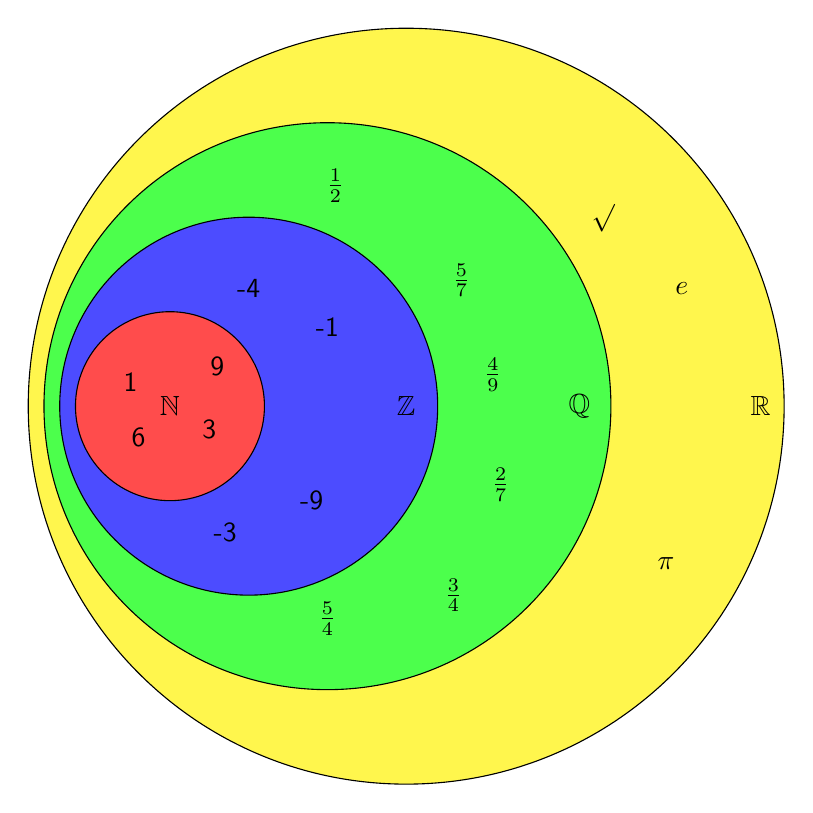
\begin{tikzpicture}[font=\sffamily]
  % Zentrale Punkte für die Positionierung der Beschriftungen
  \coordinate (N) at (-3,0);
  \coordinate (Z) at (0,0);
  \coordinate (Q) at (2.2,0);
  \coordinate (R) at (4.5,0);
  \coordinate (C) at (6.6,0);
  
  % Konzentrische Kreise
  \draw[fill=yellow!70] (0,0) circle (4.8cm); % R
  \draw[fill=green!70] (-1,0) circle (3.6cm); % Q
  \draw[fill=blue!70] (-2,0) circle (2.4cm);  % Z
  \draw[fill=red!70] (-3,0) circle (1.2cm);   % N
  

  % Beschriftungen
  \node at (N) {$\mathbb{N}$};
  \node at (Z) {$\mathbb{Z}$};
  \node at (Q) {$\mathbb{Q}$};
  \node at (R) {$\mathbb{R}$};
  
   % Zahlenbeispiele
  % Natürliche Zahlen N
  \node at (-3.5,0.3) {1};
  \node at (-2.5,-0.3) {3};
  \node at (-3.4,-0.4) {6};
  \node at (-2.4,0.5) {9};

  % Ganze Zahlen Z
  \node at (-1,1) {-1};
  \node at (-2,1.5) {-4};
  \node at (-1.2,-1.2) {-9};
\node at (-2.3,-1.6) {-3};
  
  % Rationale Zahlen Q
  \node at (-0.9,2.8) {$\frac{1}{2}$};
  \node at (0.6,-2.4) {$\frac{3}{4}$};
  \node at (-1,-2.7) {$\frac{5}{4}$};
  \node at (1.1,0.4) {$\frac{4}{9}$};
  \node at (1.2,-1) {$\frac{2}{7}$};
  \node at (0.7,1.6) {$\frac{5}{7}$};
  
  % Reelle Zahlen R
  \node at (2.5,2.4) {$\sqrt{}$};
  \node at (3.3,-2) {$\pi$};
  \node at (3.5,1.5) {$e$};
  
\end{tikzpicture}
\end{figure}
\begin{itemize}
	\item [$\mathbb{N}$] Die Zahlenmenge der natürlichen Zahlen beinhaltet alle positiven Zahlen, die kein Dezimalbruch sind
	\item [$\mathbb{Z}$] Die Zahlenmenge der ganzen Zahlen beinhaltet alle Zahlen der vorherigen Zahlenmenge inklusive negativer Zahlen
	\item [$\mathbb{Q}$] Die Zahlenmenge der rationaler Zahlen beinhaltet alle Zahlen der vorherigen Zahlenmenge inklusive Dezimalbrüche und Brüche
	\item [$\mathbb{R}$]  Die Zahlenmenge der reelen Zahlen beinhaltet alle Zahlen der vorherigen Zahlenmenge inklusive Zahlen wie $pi$, $e$ und 
\end{itemize}
\pagebreak

% GTR %
\section{GRT}\label{sec:GTR}
\subsection{Eintragen einer Funktion}\label{sec:Eintragen einer Funktion}
\begin{paracol}{2}
\begin{flushleft}
Mit dem Grafiktaschenrechner kann man sich die Graphen verschiedener Funktionen anzeigen lasse. Dazu geht man zuerst auf und trägt dort unter  y1, y2,y3, die gewünschten Funktionen ein. Funktionen, die gezeichnet werden sollen, müssen ausgewählt werden, indem auf das Gleichheitszeichen gedrückt wird und dieses schwarz hinterlegt bleibt. 

\end{flushleft}	
\switchcolumn
\begin{flushright}
\includegraphics[width=6cm]{Media/GRT/Visualisierung/einsetzen_eines_wertes_in_Funktion/einsetzen_eines_wertes_in_Funktion}
\end{flushright}
\end{paracol}

\subsection{Anpassen des Fensterbereiches des Graphen}\label{sec:Anpassen des Fensterbereiches des Graphen}
\begin{paracol}{2}
\begin{flushleft}
Um das Window anzupassen, in dem der Graphen darsgestellt wird, muss man zuerst \gtr{2nd} und \gtr{window} drücken. Anschließend unterscheidet man zwischen den Werten. 
	\begin{itemize}
		\item[] \texttt{Xmin} Dieser Wert bezeichnet den mindest Wert auf der X-Achs, der zu sehen sein wird
		\item[] \texttt{Xmax} Dieser Wert bezeichnet den maximalen Wert, der auf der X-Achse zu sehen sein wird.
	\end{itemize}

\end{flushleft}	
\switchcolumn
\begin{flushright}
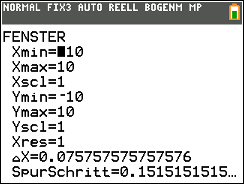
\includegraphics[width=6cm]{Media/GRT/Visualisierung/Fensterbereich_anpassen/fenster}
\end{flushright}
\end{paracol}

\begin{itemize}
	\item[] \texttt{Xscl} Dieser Wert bezeichnet die Schrittlänge auf der X-Achse 
	\item[] \texttt{Ymin} Dieser Wert bezeichnet den minimal zu sehenden Y-Wert auf der Y-Achse
	\item[] \texttt{Ymax} Dieser Wert bezeichnet den maximalen zu sehenden Y-Wert auf der Y-Achse
	\item[] \texttt{Yscl} Dieser Wert bezeichnet die Schrittlänge auf der Y-Achse
\end{itemize} Beim dem Angeben der Werte ist darauf zu achten, dass jegliche negativen Werte nicht mit dem Rechenminus, sonder mit dem Vorzeichenminus angegeben werden. Wurde der Window Bereich eingestellt, kann man im Anschluss mit der Taste \gtr{graph} zu der Ansicht des Koordinatensystems wechseln.
Ist der Graph nicht zu sehen, kann man auch über \gtr{zoom} und anschließend \texttt{zoomStandart} sich wieder die ursprüngliche Einstellung herstellen. 

\subsection{Komplett Reset}\label{sec:Komplett Reset}
\begin{paracol}{2}
\begin{flushleft}
	Sollte der Fall eines Fehlers auftreten, so ist das maximalinvasivste ein Reset des Taschenrechners, welcher durch die Tagenfolge \gtr{2nd} und \gtr{+}. Anschließend wählt man \texttt{reset} aus.
\end{flushleft}
\switchcolumn
\begin{flushright}
	\includegraphics[width=6cm]{Media/GRT/Visualisierung/komplett_reset/komplett_reset}
\end{flushright}	
\end{paracol}

\subsection{Einsetzen von Werten in eine Funktion}\label{sec:Einsetzen von Werten in eine Funktion}
\begin{paracol}{2}
\begin{flushleft}
	Mit den Tasten \gtr{2nd} und \gtr{trace} lässt sich das Menü zum Berechnen von verschiedenen Funktionsberechnungen aufrufen. Wählt man nun hier \texttt{1} , so kann man einen Wert in eine Funktion einsetzten für die Variable $x$.\\
	Die Dokumentation erfolgt hierbei wie folgt: \\
	$\mathrm{value}(y_1,\mathit{Wert}) \rightarrow y=\mathit{Wert}$
	
\end{flushleft}
\switchcolumn
\begin{flushright}
	\includegraphics[width=6cm]{Media/GRT/Visualisierung/einsetzen_eines_wertes_in_Funktion/einsetzen_eines_wertes_in_Funktion}
\end{flushright}
\end{paracol}
\pagebreak
\subsection{Schnittpunkt ermitteln}\label{sec:Schnittpunkt ermitteln}

\begin{paracol}{2}
\begin{flushleft}
	Mit den Tasten \gtr{2nd} und \gtr{trace} lässt sich das Menü zum berechnen von verschiedenen Funktionsberechnungen aufrufen. Wählt man \texttt{5}, so kann man den Schnittpunkt von zwei Funktionen berechnen lassen. Hierfür muss man im ersten Schritt die erste Funktion auswähle und anschließend die zweiten und den ungefähren Schnittpunkt der beiden Funktionen.
	$\textrm{intersect}(y_1,y_2)\rightarrow \quad x=\quad y=$
\end{flushleft}
\switchcolumn
\begin{flushright}
	\includegraphics[width=6cm]{Media/GRT/Visualisierung/Schnittpunkt_ermitteln/Schnittpunkt_ermitteln_1}
	\includegraphics[width=6cm]{Media/GRT/Visualisierung/Schnittpunkt_ermitteln/Schnittpunkt_ermitteln_2}
	\includegraphics[width=6cm]{Media/GRT/Visualisierung/Schnittpunkt_ermitteln/Schnittpunkt_ermitteln_3}
	\includegraphics[width=6cm]{Media/GRT/Visualisierung/Schnittpunkt_ermitteln/Schnittpunkt_ermitteln_4}
\end{flushright}
\end{paracol}

\subsection{Lösen von Gleichungen}\label{sec:Loesen von Gleichungen}
Ist eine Gleichung mit einer Unbekannten in der Grundform $=0$ gegeben, so kann man diese leicht mit dem GTR lösen.

\begin{paracol}{2}
	\begin{flushleft}
	Zuerst erfolgt das Eintragen der Funktion indem, indem die Funktionen eingetragen werden. Dieses wird aufgerufen, indem man die Taste \gtr{y=} drückt.
		Anschließend drückt man die Taste \gtr{graph}, um sich den Graphen anzeigen zu lassen. 
	\end{flushleft}
\switchcolumn
	\begin{flushright}
	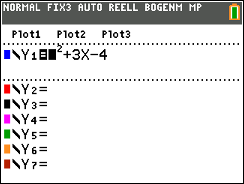
\includegraphics[width= 6cm]{Media/GRT/Visualisierung/loesen_gleichung/loesen_gleichung_1.png}
		\end{flushright}
\end{paracol}


\begin{paracol}{2}
	\begin{flushleft}
	Um nun die Gleichung nach Null aufzulösen, wählt man \gtr{2nd} und \gtr{trace} und wählt Null aus.
		\end{flushleft}
\switchcolumn
	\begin{flushright}
	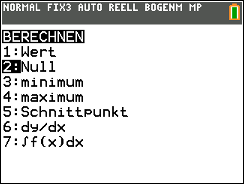
\includegraphics[width= 6cm]{Media/GRT/Visualisierung/loesen_gleichung/loesen_gleichung_2.png}
		\end{flushright}
\end{paracol}

\begin{paracol}{2}
	\begin{flushleft}
	Anschließend müssen die Grenzen bestimmt werden, indem der Taschenrechner die Nullstellen bestimmen soll. Das Wählen der ersten Grenze sollte überhalb der ersten Nullstelle geschehen.
		\end{flushleft}
\switchcolumn
	\begin{flushright}
	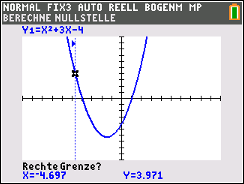
\includegraphics[width= 6cm]{Media/GRT/Visualisierung/loesen_gleichung/loesen_gleichung_3.png}
		\end{flushright}
\end{paracol}

\begin{paracol}{2}
	\begin{flushleft}
	Das Wählen der rechten Grenze geschieht unterhalb der Nullstelle.
		\end{flushleft}
\switchcolumn
	\begin{flushright}
	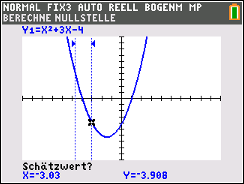
\includegraphics[width= 6cm]{Media/GRT/Visualisierung/loesen_gleichung/loesen_gleichung_4.png}
		\end{flushright}
\end{paracol}

\begin{paracol}{2}
	\begin{flushleft}
	Um schlussendlich die Nullstellen zu bestimmen müssen die Grenzen bestätigt werden. Anschließend zeigt der Taschenrechner die Nullstellen an.
	%TODO Eine Lösung finden die Dokumentation hier zu schreiben, ohne dass ein Fehler auftritt
	%\[(y_1)\rightarrowx=1\quad y=0\]
		\end{flushleft}
\switchcolumn
	\begin{flushright}
	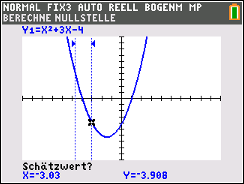
\includegraphics[width= 6cm]{Media/GRT/Visualisierung/loesen_gleichung/loesen_gleichung_4.png}
		\end{flushright}
		
\end{paracol}
\pagebreak

\subsection{Lösen von Gleichungen ohne Graph}\label{sec:Loesen von Gleichungen ohne Graph}
Nicht nur das Lösen nach Null ist möglich mit dem Taschenrechner. Genauso lässt sich eine klassische Gleichung äquvalent umformen mit dem folgenden Vorgehen.

\begin{paracol}{2}
	\begin{flushleft}
	Zunächst navigiert man mit der Taste \gtr{math} auf das \texttt{math} Menu und wählt dort ganz unten die Option \texttt{Numeric Solver} aus. 
	\end{flushleft}	
\switchcolumn
	\begin{flushright}
		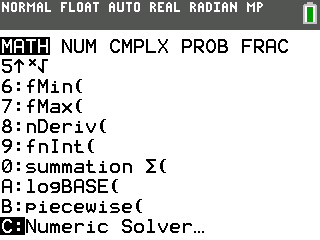
\includegraphics[width=6cm]{Media/GRT/Visualisierung/Gleichung_loesen_aequivalent/Gleichung_loesen_aequivalent_1.png}
	\end{flushright}
\end{paracol}

\begin{paracol}{2}
	\begin{flushleft}
	Nun kann man jeweils die beiden Gleichungen in die Felder \texttt{EQ1} und \texttt{EQ2}
	\end{flushleft}	
\switchcolumn
	\begin{flushright}
		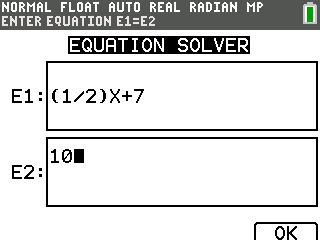
\includegraphics[width=6cm]{Media/GRT/Visualisierung/Gleichung_loesen_aequivalent/Gleichung_loesen_aequivalent_3.png}
	\end{flushright}
\end{paracol}

\begin{paracol}{2}
	\begin{flushleft}
	Abschließend drückt man die Taste unter \texttt{ok}, worauf man in dem folgenden Fenster die Grenzen bestimmen kann. Dies ist nur relevant für Gleichungen, die mehrere Ergebnisse liefern können. 
	\end{flushleft}	
\switchcolumn
	\begin{flushright}
		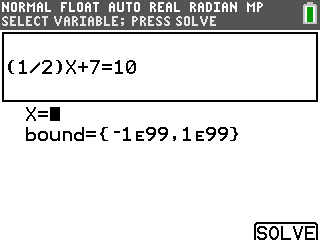
\includegraphics[width=6cm]{Media/GRT/Visualisierung/Gleichung_loesen_aequivalent/Gleichung_loesen_aequivalent_4.png}
	\end{flushright}
\end{paracol}
\begin{paracol}{2}
	\begin{flushleft}
	Abschließend bestätigt man wieder mit der Taste, die unter \texttt{ok} liegt, und erhält ein Ergebnis. 
	\end{flushleft}	
\switchcolumn
	\begin{flushright}
		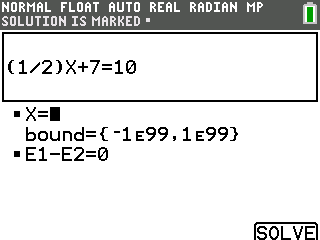
\includegraphics[width=6cm]{Media/GRT/Visualisierung/Gleichung_loesen_aequivalent/Gleichung_loesen_aequivalent_5.png}
	\end{flushright}
\end{paracol}
\subsection{Ableitungsgraph bestimmen}\label{sec:Ableitungsgraph bestimmen}
Auch der Ableitungsgraph lässt sich mit dem Taschenrechner problemlos bestimmen, indem man den \texttt{nDeriv} Befehl anwendet. 
\begin{paracol}{2}
\begin{flushleft}
	Zuerst benötigt man einen bereits eingetragenen Graphen in der Graphenübersicht bei \gtr{y=} und navigiert auf die nächste freie Funktion.
\end{flushleft}
\switchcolumn
\begin{flushright}
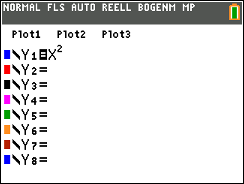
\includegraphics[width=6cm]{Media/GRT/Visualisierung/ableitung_bestimmen/ableitung_bestimmen_1.png}
\end{flushright}
\end{paracol}

\begin{paracol}{2}
\begin{flushleft}
	Nun drückt man die Taste \gtr{math} und wählt aus dem Menu den \texttt{nDeriv} Befehl aus (Herkunft engl. Derivation). Anschließend fügt der Taschenrechner den \texttt{nDrevi} in das Feld der Funktion ein
\end{flushleft}	
\switchcolumn
\begin{flushright}
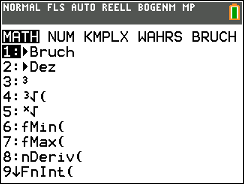
\includegraphics[width=6cm]{Media/GRT/Visualisierung/ableitung_bestimmen/ableitung_bestimmen_2.png}
\end{flushright}
\end{paracol}

\begin{paracol}{2}
\begin{flushleft}
	Hier muss nun die umpunkteten Feldern ein Wert eingetragen werden. Der Bruch wird wie folgt definiert $\frac{d}{dx}$. In die Klammer wird die Funktion deren Ableitung gewünscht ist eingetragen mit der Taste \gtr{alpha} und \gtr{trace} drauf öffnet sich Menu aus Funktionen, die dort eingesetzt werden können. Zuletzt wird in dem hintersten Feld erneut $x$ eingetragen. Drückt man nun erneut \gtr{graph}, so erhält man den Ableitungsgraph der Funktion.
	\end{flushleft}	
\switchcolumn
\begin{flushright}
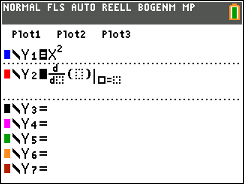
\includegraphics[width=6cm]{Media/GRT/Visualisierung/ableitung_bestimmen/ableitung_bestimmen_3.png}
\end{flushright}
\end{paracol}
\pagebreak

\pagebreak
\subsection{Unbekannte Intervallgrenzen eintragen}\label{sec:Unbekannte Intervallgrenze eintragen}
Um eine bekannten Flächeninhalt mit einer unbekannten Intervallgrenze zu berechnen, geht man wie folgt vor.
\begin{paracol}{2}
\begin{flushleft}
	Eintragen der Ausgangsfunktion in das Funktionsmenü bei \gtr{y=}
\end{flushleft}	
\switchcolumn
\begin{flushright}
\begin{figure}
	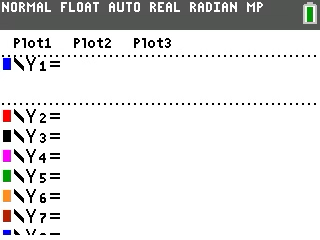
\includegraphics[width=6cm]{Media/GRT/Visualisierung/unbekannte_intervallgrenze/unbekannte_intervallgrenze_1.png}
	\caption{\link{https://youtu.be/it9pl_ZB9wc}{Visualisierung}}
\end{figure}
\end{flushright}
\end{paracol}
Anschließend muss nun das Integral eingetragen werden. Hierfür drückt man zunächst auf die Taste \gtr{math} und wählt anschließend die Option \texttt{fnInt()} aus. Nun müssen die Integralgrenzen eingefügt werden. Die erste bekannte Intervallgrenze wird unten eingefügt, während die unbekannte mit $x$ ersetzt wird. Hiernach muss die Funktion eingetragen werden, so wie die Variable, nach der hier aufgelöst wird. Abschließend kann die Taste \gtr{graph} gedrückt werden. Auf dem Graphen Fenster ist nun die Stammfunktion zu sehen.
\pagebreak
\subsection{Berechnung nicht-orientierter Flächen}\label{sec:Berechnung nicht-orientierter Flaechen}
Um anstatt mit orientierten Flächen mit dem reinen Flächeninhalt zu rechnen, muss mit dem Betrag gerechnet werden.
\begin{paracol}{2}
\begin{flushleft}
	Zunächst müssen die Nullstellen mit dem Befehl \texttt{zero} ermittelt werden. Hierfür geht man auf \gtr{2nd} und \gtr{trace}, wählt dort \texttt{zero} aus und gibt nun rechts und links die Grenzen der Nullstelle an. Abschließend drückt man \texttt{Enter} und erhält die x-Koordiante. Dieser Vorgang ist Abhängig von der Anzahl der Nullstellen und muss ggf. mehr als zwei Mal wiederholt werden. 
\end{flushleft}	
\switchcolumn
\begin{flushright}
	\begin{figure}
		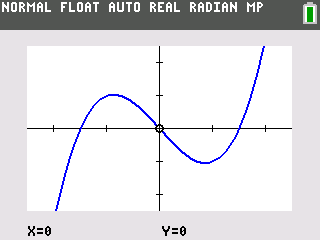
\includegraphics[width=6cm]{Media/GRT/Visualisierung/berechnung_nichtOrientierter_Flacheninhalt/berechnung_nichtOrientierter_Flacheninhalt_1.png}
		\caption{\link{https://youtu.be/MD6kzV_FIQc}{Visualisierung}}

	\end{figure}
	\end{flushright}
\end{paracol}
Anschließend muss nun der Flächeninhalt zwischen dem Graphen und der x-Achse berechnet werden mithilfe der Betragsstriche. Hierfür benutzt man die im vorherigen Schritt berechneten Nullstellen als Intervallgrenzen und berechnet den jeweiligen Flächeninhalt. Diese werden anschließend addiert, worauf man den gesamten Flächeninhalt des Graphen in einem Intervall hat. 
	Die Druchführung der Addition darf nicht im Bereich der Funktion durchgeführt werden, da hierbei sich nur einen Gleichung ergibt, welche als lineare dargestellt wird. Um nun ein Integral einzutragen verwendet man \gtr{math} und wählt die Option \texttt{fnInt()} an. Anschließend kann man die Intervallgrenzen (berechneten Nullstellen) eintragen. Um nun den Betrag einer Funktion zu verwenden, muss man auf \gtr{math} drücken und dort mit den Pfeiltasten auf die Kategorie \texttt{NUM} navigieren. Dort wählt man \texttt{abs()} aus und bestätigt mit \texttt{Enter}. 
\pagebreak
\subsection{Flächeninhalt zwischen zwei Funktionen berechnen}\label{sec:Flaecheninhalt zwischen zwei Funktionen berechnen}
Bei berechnen von einem Flächeninhalt zwischen zwei Funktionen stellt sich ein ähnliches Problem Problem heraus wie bei berechnen des Flächeninhalts mit der x-Achse.
\begin{paracol}{2}
	\begin{flushleft}
	Um den Flächeninhalt mit dem GTR zu berechnen, bildet man zunächst die Differenzenfunktion, indem man sich bei Funktionen in der Funktionsübersicht einträgt und anschließend eine weitere definiert. Diese Funktion subtrahiert die beide vorherigen Funktionen von einandern. 
	\end{flushleft}
\switchcolumn
	\begin{flushright}
		\begin{figure}
			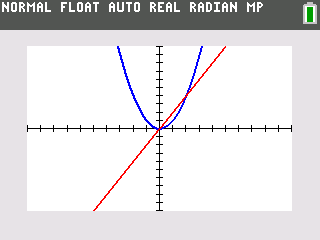
\includegraphics[width=6cm]{Media/GRT/Visualisierung/Flaecheninhalt_zwischen_zwei_Funktionen_berechnen/Flaecheninhalt_zwischen_zwei_Funktionen_berechnen.png}
		\caption{\link{https://youtu.be/y-6UFVmVIOE}{Visualsisierung}}
		\end{figure}
	\end{flushright}
\end{paracol}
\pagebreak
\subsection{Regression}\label{sec:Regression}
Die Regression ist ein Verfahren, bei dem Zusammenhänge zwischen Abhängigkeiten einer oder mehrere Variablen analysiert werden. Beim GTR gibt es verschiedene Arten, die für verschiedenen Graphen sind. Diese Arten sind spezifisch für spezifische Graphen gedacht, weswegen das wählen dieser sorgfältig erfolgen sollte. 

\begin{paracol}{2}
\begin{flushleft}
	Um mithilfe von Regression eine Funktionsgleichung zu bestimmen geht man über \gtr{stat} in das \texttt{STAT}-Menu.
\end{flushleft}	
\switchcolumn
\begin{flushright}
	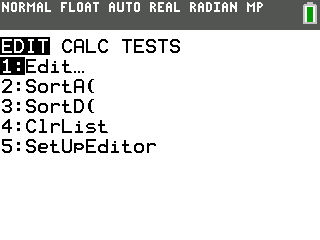
\includegraphics[width=6cm]{Media/GRT/Visualisierung/Regression/Regression_1.png}
\end{flushright}
\end{paracol}

\begin{paracol}{2}
	\begin{flushleft}
	Anschließend wählt man Edit aus und kommt in die Listenansicht. In dieser müssen nun mindestens zwei verschiedene Punkte eingetragen werden. In der ersten Spalte befinden sich hierbei die $x$-Wert und in der zweiten die $y$-Werte. 
	\end{flushleft}	
\switchcolumn
	\begin{flushright}
		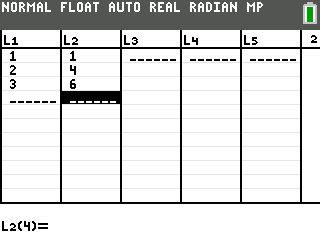
\includegraphics[width=6cm]{Media/GRT/Visualisierung/Regression/Regression_5.png}
	\end{flushright}
\end{paracol}

\begin{paracol}{2}
	\begin{flushleft}
	Sind die Werte eingetragen, so drückt man erneut \gtr{stat} und navigiert mit den Pfeiltaste in das \texttt{Calc} Menu. Dort wählt man\texttt{QuadReg} aus und bestätigt.
	\end{flushleft}	
\switchcolumn
	\begin{flushright}
		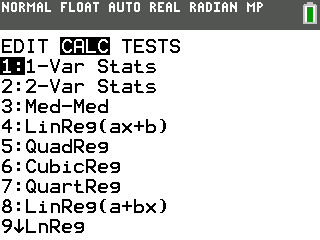
\includegraphics[width=6cm]{Media/GRT/Visualisierung/Regression/Regression_3.png}
	\end{flushright}
\end{paracol}

\begin{paracol}{2}
	\begin{flushleft}
	Bestätigt man erneut kommt man in eine Bestätigungsansicht, wo die jeweiligen Listen erneut ausgewählt werden müssen. Bestätigt man dies, so erhalt man 
	\begin{center}
			\texttt{LinReg}\\
			\end{center}
			\texttt{y=ax+c}\\
			\texttt{a=-05}\\
			\texttt{c=3}
	\end{flushleft}	
\switchcolumn
	\begin{flushright}
		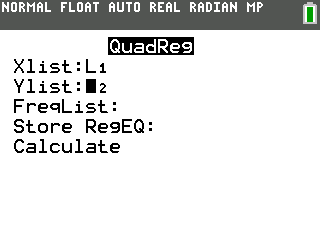
\includegraphics[width=6cm]{Media/GRT/Visualisierung/Regression/Regression_4.png}
		
	\end{flushright}
\end{paracol}
\pagebreak













% Definition Terme
\section{Terme}\label{sec:Terme}
Ein Term ist ein Rechenausdruck, der aus verschiedenen Faktoren und Summanden besteht. Mit einem Term können reelle Sachverhalte oder mathematische Zusammenhänge ausgedrückt werden.

\begin{beispiel}
\begin{enumerate}
	\item Maren kauft zwei Äpfel und drei Bananen
\[\Rightarrow2a+2b\]
\item Zu dem dreifachen einer Unbekannten wird das fünfache einer weiteren Unbekannten addiert
\[\Rightarrow 3x+5y\]
\end{enumerate}
\end{beispiel}

\subsection{Zusammenfassen von Termen}\label{sec:Zusammenfassen von Termen}
Ist ein Term gegeben, so kann man alle Variablen mit dem gleichen Namen zusammenfassen und so den Term vereinfachen. Hierbei werden die Terme der gleichen Sorte zusammengefasst. Weitere Themen zum vereinfachen von Termen sind in den Rechengesetzten zu finden.
%todo Referenz zu Distributiv- Kommutativ- und Assoziativgesetzt

\begin{beispiel}
	\[\color{red}{2a}\color{blue}{-3b} \color{red}{+5a}\color{blue}{-7b}\color{black}{=}\color{red}{7a}\color{black}{+}\color{blue}{-10b} \]
\end{beispiel}
\subsubsection{Vereinfachung mit Faktorisierung}
Nicht nur lassen sich Terme der gleichen ''Sorte'' wie in dem oberen Beispiel zusammenfassen, sondern auch mit der Hilfe der Faktorrisierung. Dies bedeutet, dass man durch Ausklammern der Variablen die Koeffizienten zusammenfassen kann. 

\begin{beispiel}
\begin{align*}
	2a+5a-3b-7b\\
	=a(2+5)+b(-3-7)\\
	=7a+b(-10)
\end{align*}	
\end{beispiel}


% Rechengesetzte
\pagebreak

\section{Rechengesetze}\label{sec:Rechengesetzte}
Die Rechengesetze sind grundlegend für die Anwendung vieler Rechenverfahren. Sie beschreiben Grundlegende Regeln, die ausnahmslos gelten.

\subsection{Distributivgesetz}\label{sec:Distributivgesetzt}
Das Distributivgesetz ist auch unter dem Namen Verteilungsgesetz bekannt. Hierbei wird ein Faktor vor einer Klammer auf alle Inhalte einer Klammer verteilt. 

\begin{beispiel}
	\[a\cdot(b+c)=a\cdot b+a\cdot c\]
\end{beispiel}
\subsection{Erweitertes Distributivgesetz}\label{sec:Erweitertes Distributivgesetz}
Das erweiterte Distributivgesetz wird auf die Multiplikation von zwei Klammern miteinander, so kann man diese auflösen, indem man das einfache Distributivgesetz mehrfach hintereinander anwendet. 

\begin{beispiel}
	\begin{enumerate}
		\item Mit Variablen: \[(a+b)\cdot(c+d)=(a+b)\cdot c+(ac+b)\cdot d=ac+bc+ad+ad+bd\]
		\item Mit Zahlen: \[(3a-6c)\cdot (-2a+3b)=-6a^2+9ab+12ca-18cb\]
	\end{enumerate}
\end{beispiel}
\pagebreak
\subsection{Faktorisieren}\label{sec:Faktorisieren}
In manchen Fällen ist es sinnvoll, einen Term mit einem Produkt zu verwandeln. Diesen Vorgang nennt man Faktorisieren. Dabei sucht man seine Variable oder einen Teiler, der in jedem Summanden des Terms vorkommt und zieht diesen aus dem Term heraus, indem man das Distributivgesetz ''rückwärts'' anwendet.
Man schreibt: $\color {red}a\color {black}b+\color {red}a\color {black}c+\color {red}a\color {black}d=\color {red}a\color {black}\cdot b+\color {red}a\color {black}\cdot c+\color {red}a\color {black}\cdot d=\color {red}a\color {black}\cdot(b+c+d)$

\begin{beispiel}
	\begin{enumerate}
		\item 
			\begin{align*}
				&3\color{red}a\color{black}-6\color{red}a\color{black}b+4\color{red}a\color{black}c\\
				&=\color{red}a\color{black}\cdot3+\color{red}a\color{black}\cdot6b+\color{red}a\color{black}\cdot4c\\
				&=\color{red}a\color{black}\cdot(3-6b+4c)
			\end{align*}
		\item 
			\begin{align*}
				&6ac-8ab+10a^2\\
				&=2a\cdot 3c-2a\cdot 4b+2a\cdot5a\\
				&=(3c-4b+5a)\cdot2a
			\end{align*}
		\item 
			\begin{align*}
				&x-2x^2+3x^3\\
				&=x\cdot 1-x\cdot 2x+x\cdot 3x^2
			\end{align*}
	\end{enumerate}
\end{beispiel}
\pagebreak




\section{Binomische Formeln}
Für bestimmt Anwendungen des erweiterten Distributivgesetzes wird die binomische Formel verwendet. Hierbei unterscheidet man im wesentlichen in drei Typen der binomischen Formel. Sie sind von Nutzen beim vereinfachen von Termen und sollten schnellstmöglich erkannt werden beim Rechnen. 
\begin{itemize}
	\item 1. binomische Formel \[(a\color{red}+\color{black}b)^2=a^2\color{red}+\color{black}2ab+b^2\]
	\item 2. binomische Formel \[(a\color{red}-\color{black}b)^2=a^2\color{red}-\color{black}2ab+b^2\]
	\item 3. binomische Formel \[(a+b)\cdot (a-b)=a^2-b^2\]
\end{itemize}

% Brüche
\section{Brüche}\label{sec:Brueche}
Brüche sind in der Mathematik grundlegenden für das Verständnis für viele Rechnungen. Dabei sind sie oftmals genauer als Dezimalbrüche, da sie, im Gegenteil zu Dezimalbrüchen, periodische Zahlen darstellen können, ohne sie Runden zu müssen. Dies bedeutet Brüche sind deutlich genauer im Vergleich zu Dezimalbrüchen. Dabei ist ein Bruch nicht anders als eine andere Darstellungsweise für eine Division.
\subsection{Termination}\label{sec:Brueche/Termination}
 Bezüglich der Termination von Brüchen gilt Folgendes.\\
\[\color{red}a:\color{blue}b\color{black}= \frac{\color{red}a}{\color{blue}b}\]
Wobei $\color{red}{a}$ bei einem Bruch als Zähler bezeichnet wird und dabei angibt, wie viele Bruchteile des Nenners gegeben sind.  $\color{blue}{b}$ ist hierbei der Nenner und bestimmt den Namen des Bruches.
\subsection{Erweitern und kürzen von Brüchen}\label{sec:Brueche/Erweitern und kuerzen von Bruechen}
In manchen Situationen ist es notwendig, den Namen eines Bruches zu verändern, aber seinen Wert beizubehalten. Hierbei liegt das Prinzip eines Verhältnisses zugrunde. So stellt ein Bruch $\frac{1}{2}$ den gleichen Sachverhalt dar, wie der Bruch $\frac{4}{8}$.
\subsubsection{Erweitern von Brüchen} Durch das Multiplizieren von Zähler und Nenner in einem Bruch mit einer Zahl wird der ursprüngliche Bruch erweitert. 
\begin{paracol}{2}
	\begin{flushleft}
	\begin{beispiel}
\[\overset{\cdot3}{\overrightarrow{\frac{\color{red}6}{7}=\frac{\color{red}18}{21}}}\]
	\end{beispiel}
	\end{flushleft}	
\switchcolumn
	\begin{flushright}
		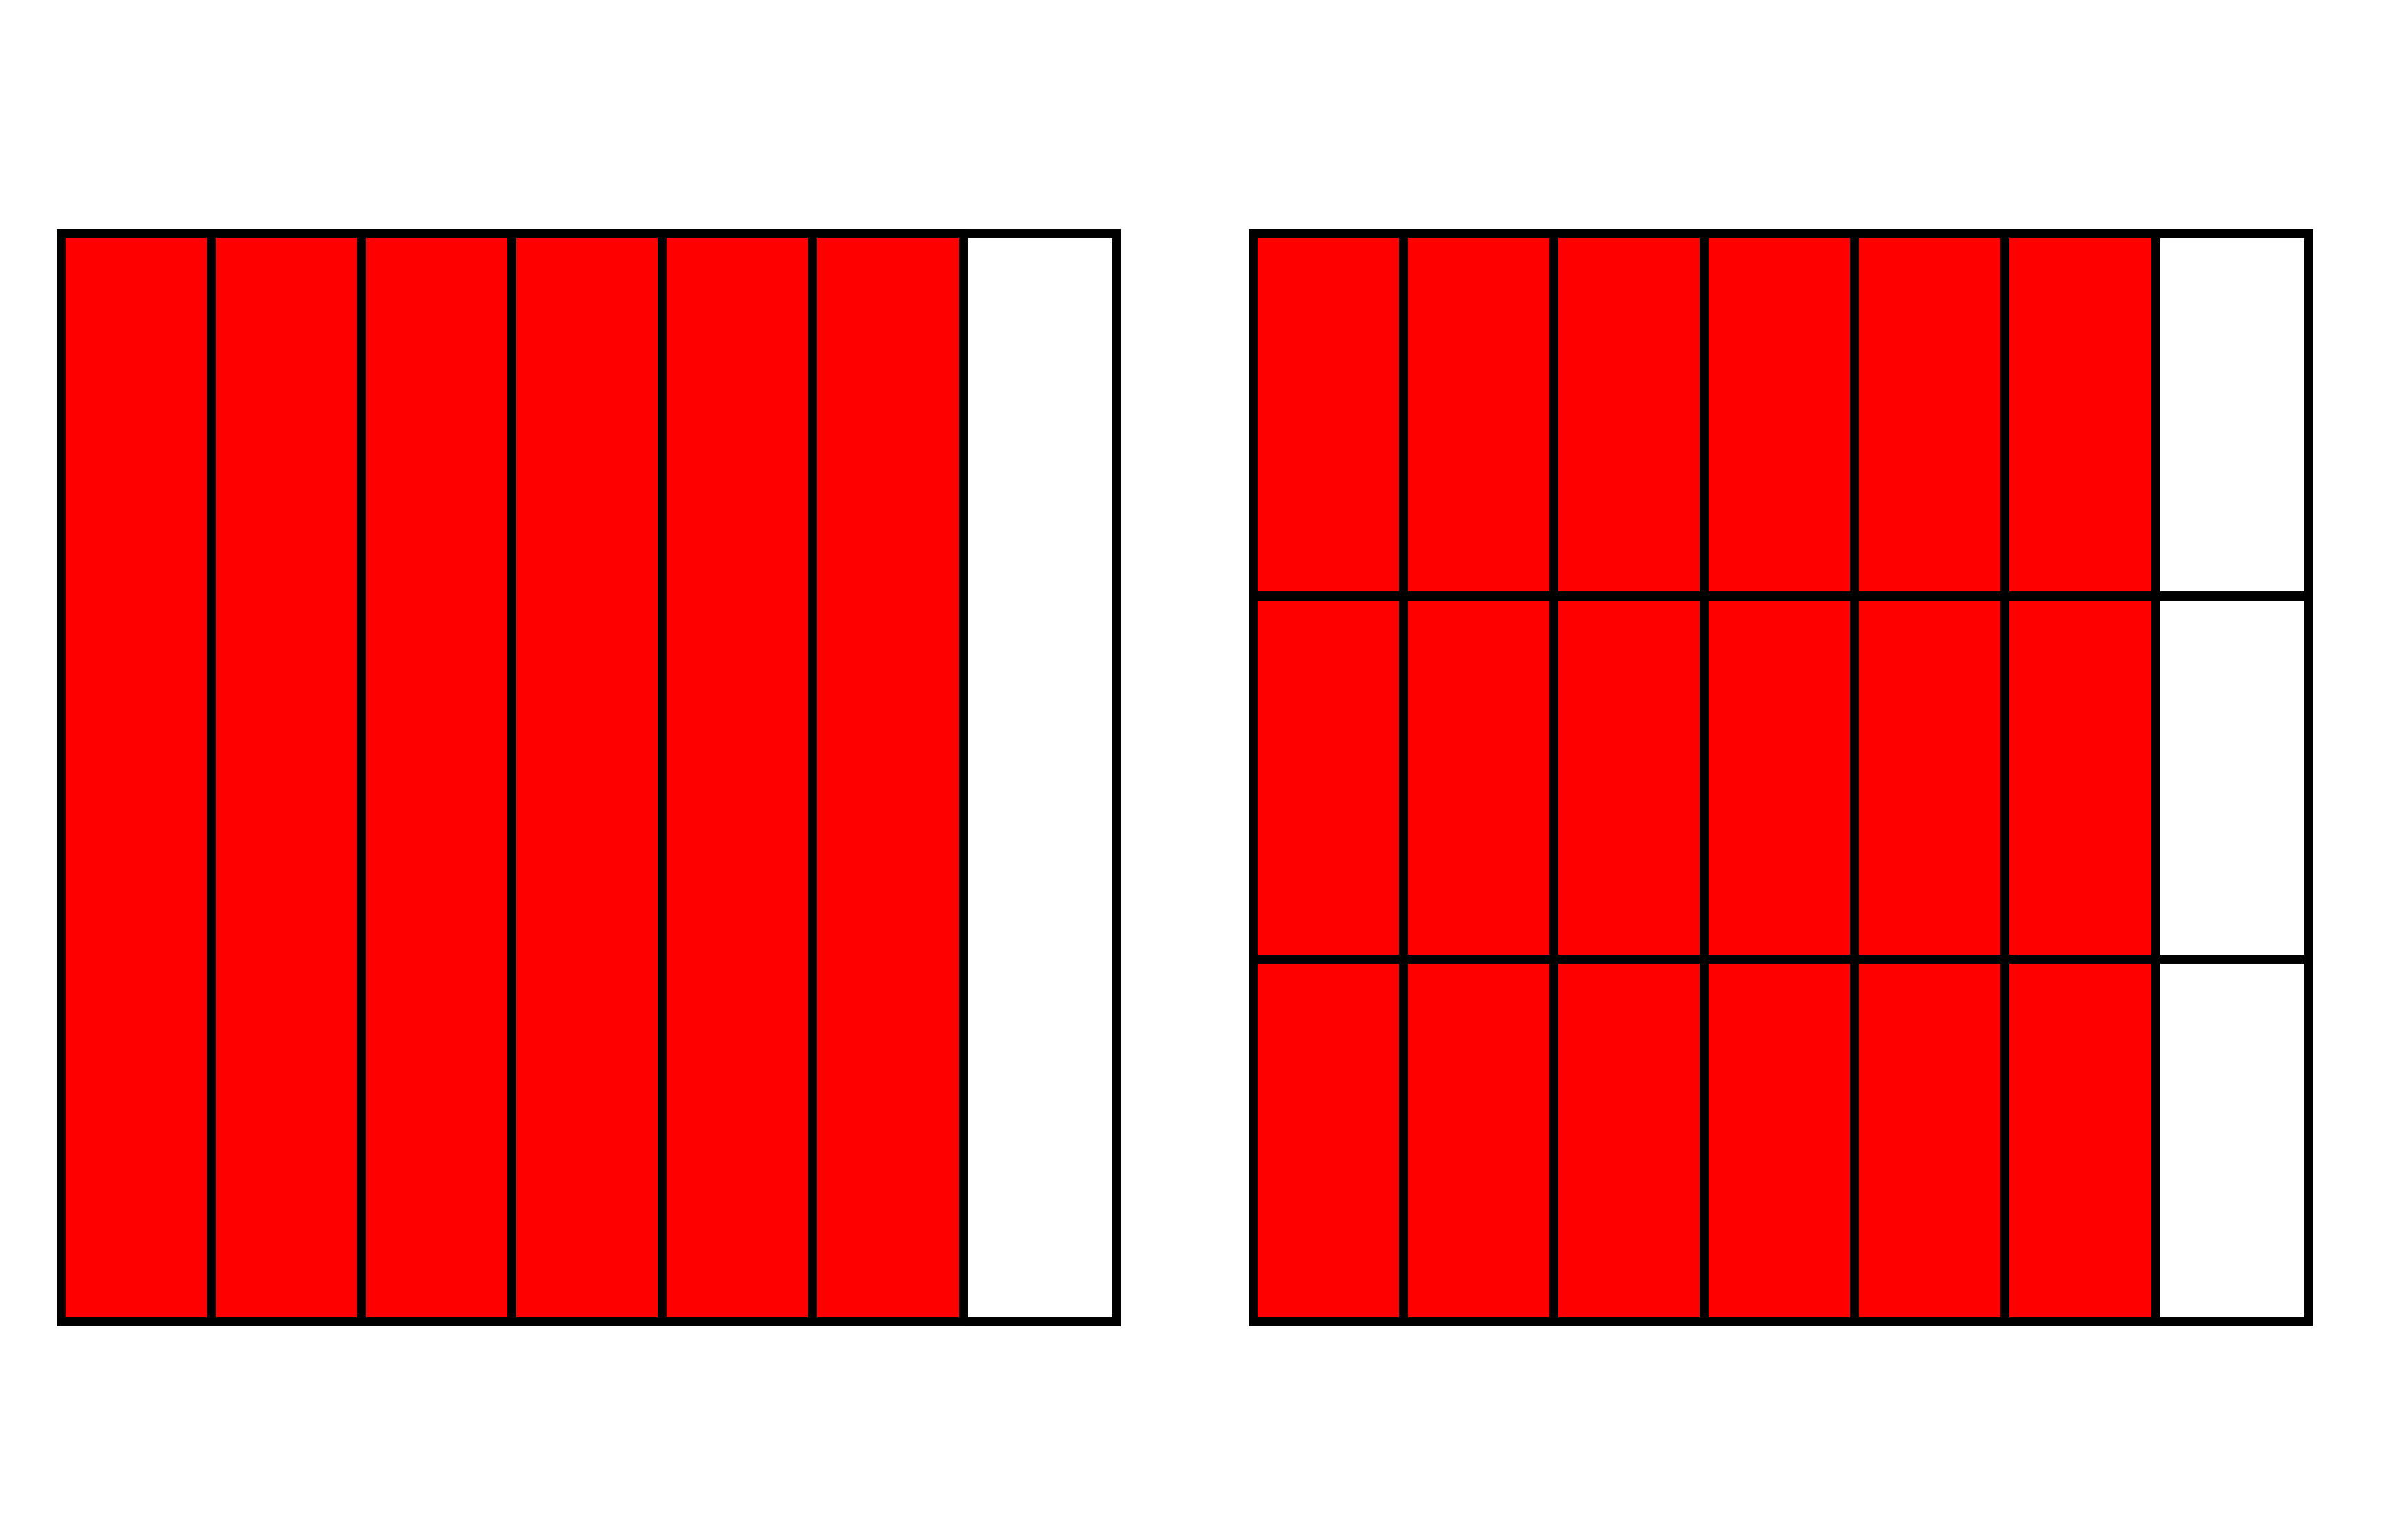
\includegraphics[width=5cm]{Media/Theorieheft-Brueche-Erweitern.png}
	\end{flushright}
\end{paracol}
\subsubsection{Kürzen von Brüchen}
Das Kürzen von Brüchen funktioniert ähnlich wie beim Erweitern, bloß umgedreht.

\begin{beispiel}
	\[\frac{\color{red}8}{28}=\frac{\color{red}2}{7}\]
\end{beispiel}

\subsubsection{Faktorisieren} Da beim Rechnen mit Brüchen ebenfalls alle Rechengesetzte gelten, kann man im Zähler und im Nenner faktorisieren.
\begin{beispiel}
	\[\frac{5x-5}{10x-5}=\frac{5\cdot(x-1)}{5\cdot(2x-1)}=\frac{x-1}{2x-1}\]
\end{beispiel}
\subsection{Rechnen mit Brüchen}\label{sec:Brueche/Rechen mit Bruechen}
Da auch mit Brüchen in der Mathematik gerechnet wird, gelten auch die Grundrechenarten.
\subsubsection{Addition und Subtraktion} Beim addieren und subtrahieren von Brüchen, muss darauf geachtet werden, dass beide Brüche gleichnamig sin. 

\begin{beispiel}
	\begin{align*}
		&\frac{2}{7}+\frac{3}{12}\\
		&=\frac{2}{7}+\frac{3}{12}\\
		&= \frac{24}{84}+\frac{21}{84}\\
		&= \frac{45}{84}
	\end{align*}	
\end{beispiel}
\subsubsection{Multiplizieren} Das Multiplizieren von Brüchen ist weniger aufwendig im Vergleich zu der Subtraktion und Addition, denn bei der Multiplikation wird lediglich der Nenner mit dem Nenner und der Zähler mit dem Zähler multipliziert.

\begin{beispiel}
	\[\frac{3}{4}\cdot\frac{7}{2}=\frac{21}{8}\]
\end{beispiel}
\subsubsection{Division} Bei der Division von Brüchen nimmt man lediglich den Kehrbruch des zu dividierenden Bruch und multipliziert ihn mit dem ersten Bruch. 

\begin{beispiel}
	\[\frac{3}{4}:\frac{4}{7} \rightarrow \frac{3}{4}\cdot \frac{7}{4}= \frac{21}{12}\]
\end{beispiel}
% Potenzen und Potenzgesetze
\section{Potzen}\label{sec:Potenzen}
Eine Potzen besteht immer aus einer Basis und einem Exponenten. Dabei gibt der Exponenten an, wie oft die Basis mit sich selbst multipliziert wird. Man schreibt $a^b$. 
\subsection{Potenzgesetzte}\label{sec:Potenzen/Potenzgesetze}
 Auch mit Potenzen kann gerechnet werden, deswegen finden gewisse Rechengesetzte auch hier eine Anwendung.
\begin{enumerate}
	\item Multiplikation von zwei Variablen mit gleicher Basis, aber mit verschiednen Exponenten. \[a^r\cdot a^s=a^{r+s}\]
	\item Dividieren von zwei Variablen mit gleicher Bais, aber verschiedene Exponenten. \[\frac{a^r}{a^s}=a^{r-s}\]
	\item Basis mit Exponent wird umklammert von einem weiteren Exponenten. \[(a^r)^s=a^{r\cdot s}\]
	\item Die Basis ist ungleich und wird mit einer anderen Baisis multipliziert, aber die Exponenten sind gleich.\[a^k \cdot b^k =(a\cdot b)^k\]
	\item Die Basis ist ungleich wird mit einer anderen Basis dividiert, aber die Exponenten sind gleich. \[\frac{a^k}{b^k}=\left(\frac{a}{b}\right)^k\]
\end{enumerate}
\subsection{Negative Exponenten umformen}\label{sec:Potenzen/Negative Exponenten umformen}
Um einen negativen Exponenten umzuformen muss dieser in ein Bruch geschrieben werden und folgt dabei folgender Form. 

\begin{beispiel}
\begin{align*}
	x^{-4}=\frac{1}{x^4}
\end{align*}
\end{beispiel}

% Wurzeln und Wurzelgesetze
\section{Wurzeln und Wurzelgesetze}
Wurzeln sind ein wesentlicher Bestandteil in der Mathematik. Das Grundkonzept hinter Wurzeln ist, dass Umkehren einer Potenz, in der eine Zahl so oft mit sich Multipliziert wird, wie der Exponent angibt. Die $n$-te Wurzel aus einer Zahl $a$ ist genau die Zahl, die $n$-mal mit sich selbst multipliziert den Wert $a$ ergibt.
Man Schreibt: $\sqrt[n]{a}$, wobei $n$ angibt, wie oft die Zahl mit sich selbst multipliziert wurde, damit sich $a$ ergibt. 

\begin{beispiel}
	\begin{align}
		\sqrt[3]{8} \Rightarrow 2\cdot 2\cdot 2&=8\\
		\sqrt[5]{243} \Rightarrow 3\cdot 3\cdot 3\cdot 3\cdot 3&=243
	\end{align}
\end{beispiel}
\subsection{Wurzelgesetze} Auch mit Wurzeln kann gerechnet werden, deswegen finden gewisse Rechengesetze auch hier einen Anwendung.
\begin{enumerate}
	\item Wurzel ziehen aus einer Division. \[\sqrt{\frac{a}{b}}=\frac{\sqrt{a}}{\sqrt{b}}\]	
	\item Wurzel ziehen aus einer Multiplikation \[\sqrt{a\cdot b}=\sqrt{a}\cdot \sqrt{b}\]
\end{enumerate}
% Gleichungen
\pagebreak
\section{Gleichungen} Eine Gleichung besteht immer aus zwei Termen, die mit einem Gleichsetzungszeichen verknüpft sind. Damit wird ausgedrückt, dass beide Seiten, der Gleichung, den gleichen Wert haben bzw. gleichschwer sind. Taucht eine oder mehrere Variablen auf einer oder beider Seiten, der Gleichung auf, so ist genau der Wert der Variable eine Lösung der Gleichung für den das Gleichheitszeichen stimmt. 
Eine Gleichung kann eine Lösung, mehrere Lösungen oder keine Lösung haben. 

\begin{beispiel}
	\begin{enumerate}
		\item Eine Lösung 
			\begin{align*}
				3x-5&=2x+3\\
				&=\{8\}
			\end{align*}
		\item mehrere Lösungen 
			\begin{align*}
				2a+b&=7\\
				&=\{(3.1);(2.3)...\}
			\end{align*}
		\item Keine Lösung
			\begin{align*}
				x^2&=-4\\
				&=\{\}
			\end{align*}
	\end{enumerate}
\end{beispiel}
\subsection{Äquivalenzumformung}
Eine Äquivalentzumformnung ist eine Umformung, die auf beiden Seiten einer Gleichung durchgeführt wird. Dabei wird die Kernaussage der Gleichung nicht verändert, die Darstellung allerdings schon.

\begin{beispiel}
	\begin{alignat*}
		3x-7&=9\qquad &| +7\\
		3x&=16 \qquad &|:3\\
		x&=\frac{16}{3}
	\end{alignat*}
\end{beispiel}
\subsection{Schema zum Lösen von Gleichungen}
Liegt eine Gleichung vor, an der der höchste Exponent $n:$$1$ ist, kann man zu der Ermittlung der Lösung wie folgt vorgehen . 
\begin{enumerate}
	\item Klammern auflösen und Zusammenfassen mit den Distributivgesetzen und der binomischen Formel.
	\item Alles mit einer Variable auf eine Seite bringen
	\item Alles ohne Variable auf die andere Seite bringen
	\item Normieren, indem man auf ein $x$ runter oder hochrechnet. 
\end{enumerate}
\setcounter{equation}{0}
\begin{beispiel}
	\begin{align}
		(x-2)&=(x+3)(x-3)\\
		x^2-4x+4x&=x^2-9\\
		-4x+4 &= -9\\
		-4x&=-13\\
		x&=\frac{13}{4}
	\end{align}
\end{beispiel}\\
Wobei in der ersten Zeile die Ausgangsgleichung steht. Anschließend folgen die Schritt, wie oben beschrieben. 
% Funktionen
\section{Funktionen}\label{sec:Die Funktion}
Eine Funktion ist eine Zuordnung aus zwei Zahlenmengen. Die Funktion $f:D\rightarrow \mathbb{R}$ mit $D\in \mathbb{R}$. Sei $a\in X$ und $b\in Y$, so bildet $a\mapsto b$ ab, und stellt somit ein Zuordnung zweier Mengen dar. Hierbei wird jedem $x$ ein $y$ zu. 
%ToDo Die Definition sollte hier nochmals überarbeitet werden

\begin{beispiel} Fährt man mit einem Auto konstant 100km/h, so kann man dies auch in einer Wertetabelle darstellen. Hierbei ist zu beachten, dass die Funktion Kilometer in Zeit darstellt.
\begin{align*}
	1 \text{ Stunde}&\mapsto100 \text{ Kilometer}\\
	2 \text{ Stunde}&\mapsto200 \text{ Kilometer}\\
	3 \text{ Stunde}&\mapsto300 \text{ Kilometer}\\
	4 \text{ Stunde}&\mapsto400 \text{ Kilometer}
\end{align*}
\end{beispiel}
\subsection{Darstellung von Funktionen}\label{sec:Die Funktion/Darstellen von Funktionen}
Setzt man in eine Funktion für das $x$ einen Wert, so erhält man den zugehörigen $y$-Wert. Dieses Wertepaar lässt sich in ein Koordinatensystem eintragen (\ref{sec:Wertetabelle_einer_Funktion_visualisiert}). Verbindet man nun die Punkte miteinand er, so entsteht der sogenannte Funktionsgraph. Auch lässt sich hierbei leicht erkennen, ob es sich überhaupt um eine Funktion, handelt. Betrachtet man die $Y$-Achse, als den obig erwähnten Wert und die $X$-Achse als Ausgangsmenge, so lässt sich feststellen, warum eine Funktion keine Zuweisung von zwei $X$-Werten haben kann.
%ToDo Warum hatt eine Funktion keine zwei X-Werte
\begin{figure}[h!]
\centering
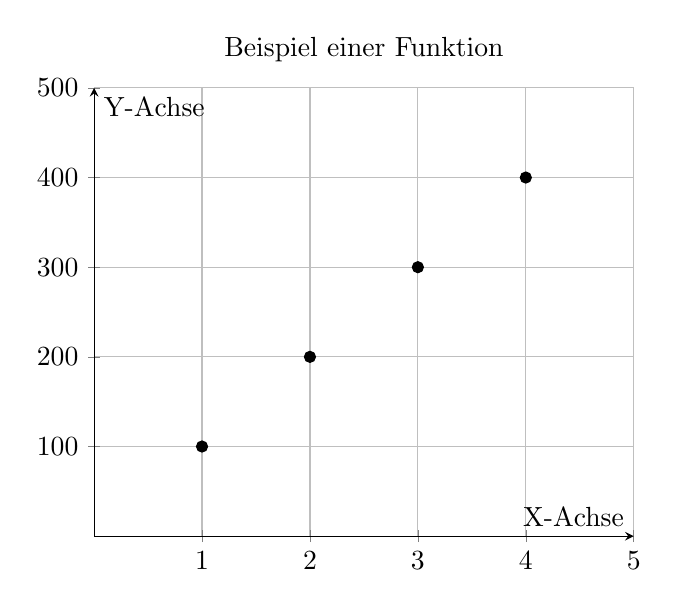
\begin{tikzpicture}
\begin{axis}[
    title={Beispiel einer Funktion},
    xlabel={X-Achse},
    ylabel={Y-Achse},
    axis lines=middle, % Zentriert die Achsen
    xmin=0, xmax=5, % Setzt die Grenzen für die X-Achse
    ymin=0, ymax=500, % Setzt die Grenzen für die Y-Achse
    grid=major, % Fügt ein Hauptgitter hinzu
]
\addplot[mark=*] coordinates {(1,100)};
\addplot[mark=*] coordinates {(2,200)};
\addplot[mark=*] coordinates {(3,300)};
\addplot[mark=*] coordinates {(4,400)};
\end{axis}
\end{tikzpicture}
\caption{Wertetabelle einer Funktion visualisiert}
\label{sec:Wertetabelle_einer_Funktion_visualisiert}
\end{figure}

 

% lineare Funktionen
\section{Lineare Funktionen}\label{sec:Lineare Funktionen}
Wird eine Funktion durch eine Gleichung in der Form $y=mx+b$ dargestellt, so spricht man von einer linearen Funktion. Dabei gibt $b$ den Schnittpunkt mit der $Y$-Achse, den sogenannten $Y$-Achsenabschnitt an. Die Variable $m$ ist die Steigung der Funktion. Hat $m$ die Form $m=\frac{a}{b}$, so gibt $b$ den Weg auf der $X$-Achse und $a$ den Weg auf der $Y$-Achse an, um von einem Punkt zu dem nächsten zu gelangen. Dies kann gut mit dem Steigungsdreieck darsgestellt werden. Beim Einzeichnen ist zu beachten, dass immer erst nach Rechts und anschließend nach oben bei potiven Zahlen und nach unten bei negativen Zahlen gegangen wird.
\subsection{Parallelität}\label{sec:Lineare Funktionen/Parallelitaet}
 Um die Eigenschaft der Parallelität zu bestimmen bei einer linearen Funktion, betrachtet man den Steigungsfaktor $m$.
Im Bezug auf Parallelität ist folgendes festzuhalten. 
\begin{align*}
	f(x)=mx+b\\
	a(x)=m_1x+b
\end{align*}
Sind die Werte, die $m$ annimmt, die selben, die $m_2$ animmt, so spricht man von einer Parallelität. Ist $m_1=m_2$, so ist $G_f||G_a$
\subsection{Orthogonalität}\label{sec:Lineare Funktionen/Orthogonalitaet}
 Im Vergleich zu der Parallelität stellt die Orthogonalität das Gegenteil dar. Eine Funktion, die zu einer anderen Orthonogal steht, bildet mit der anderen Funktion einen Schnittpunkt im 90\degree{} Winkel. Daraus folgt, dass sollte \\$m_f\cdot m_a=-1$ die Funktionen immer orthogonal zu einander stehen.
\begin{figure}[h!]
\centering
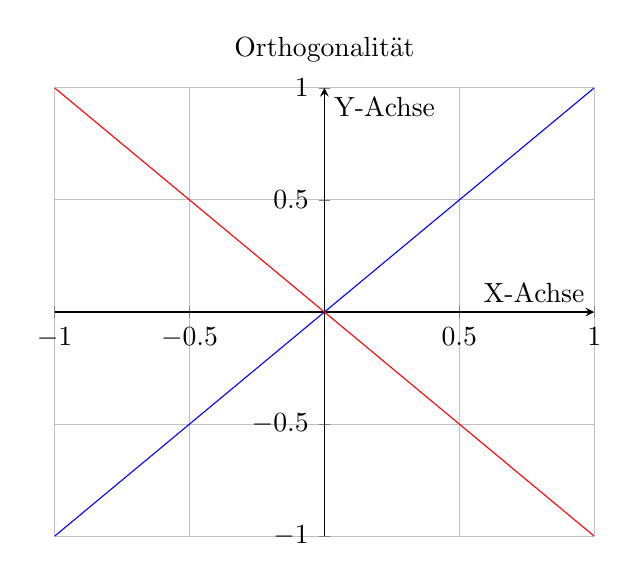
\begin{tikzpicture}
\begin{axis}[
    title={Orthogonalität},
    xlabel={X-Achse},
    ylabel={Y-Achse},
    axis lines=middle, % Zentriert die Achsen
    xmin=-1, xmax=1, % Setzt die Grenzen für die X-Achse
    ymin=-1, ymax=1, % Setzt die Grenzen für die Y-Achse
    grid=major, % Fügt ein Hauptgitter hinzu
]
\addplot+[mark=none] {x};
\addplot+[mark=none] {-x};
\end{axis}
\end{tikzpicture}
\caption{Graphisches Beispiel für Orthogonalität}
\end{figure}
\subsection{Geradengleichung bestimmen}\label{sec:Lineare Funktionen/Geradengleichung}
Bei einer linearen Funktion bei der die Steigung und ein Punkt auf einer Geraden gegeben ist, lässt sich die Funktionsgleichung leicht bestimmen. Hierzu geht man von der Grundform $f(x)=mx+b$ aus und ermittelt $b$ sowie den gesuchten Parameter. Dafür setzt man das Gegebene in die Grundform ein und bestimmt $b$ so, dass die Gleichung erfüllt ist.

\begin{beispiel}
Gesucht ist die Gerade $g_1$ mit $m=3$, die durch den Punkt $(-2;-7)$ verläuft
Dabei wird $g_1:f(x)=mx+b$ wie folgt definiert $m=3$, $x=2$, $y=-7$.
\begin{align*}
	f(x)&=mx+b\\
	-7&=-3\cdot (-2)+b\\
	-7&=6+b\\
	-13&=b
\end{align*}
Somit lautet der $Y$-Achsenabschnitt $-13$, weswegen die gesuchte Gerade wie folgt lautet: $g_1:f(x)=-3x-13$
\end{beispiel}
\subsection{Zwei-Punkt Steigungsform}\label{sec:Lineare Funktionen/Zwei-Punkt Steigungsform}
Sind von einer Geraden zwei Punkte, der Form $A(y_1;y_2)$ und $B(x_2;y_2)$, bekannt, so kann man aus diesen beiden Punkten ein Steigungsdreieck bilden. Für die Steigung gilt dann folgendes.
\begin{align*}
	m&=\frac{\text{Abstand Y-Wert}}{\text{Abstand X-Wert}}\\
	m&=\frac{y_1-y_2}{x_1-x_2}
\end{align*}

\begin{beispiel}
Die Punkte $A(1,-1)$, $B(2;3)$ sind gegeben und sollen nun mit der Zwei-Punkt Steigungsform die Steigung $m$ ergeben. 
	\begin{align*}
		m&=\frac{y_1-y_2}{x_1-x_2}\\
		m&=\frac{3-(-1)}{2-1}\\
		m&=\frac{4}{1}\\
		m&=4
	\end{align*}
	Somit ist die Steigung $m=4$ zwischen den Punkten $A\land B$
\end{beispiel}


% quadratische Funktionen
\section{Quadratische Funktionen}
Eine quadratische Funktion ist eine weitere Art der Funktionen. Sie stellt allerdings nicht wie bei den linearen Funktionen einen linearen Sachverhalt dar, sondern einen quadratischen. 
\subsection{Normalformen}
\subsubsection{Scheitelpunktform}
Der Scheitelpunkt einer quadratischen Funktion oder auch einer Parabel ist der größte bzw. kleinste Wert einer parabolischen Funktion. Die allgemeine Form der Scheitelpunktform einer quadratischen Funktion ist die folgende. 
\begin{align*}
	f(x)=a(x-d)^2+e
\end{align*}
Dabei gilt
\begin{itemize}
	\item Der Streckfaktor $a$ bestimmt, ob die Parabel nach oben ($a>0$) oder nach unten ($a<0$) geöffnet ist. Auch bestimmt er, wie die Parabel gestreckt ($|a|>0$) oder gestaucht ($(0<|a|<1)$) ist
	\item Mit dem Parameter $d$ wird angeben, wie weit die Funktion nach rechts bzw. links verschoben wird. Hierbei muss allerdings auf das Vorzeichen von $d$ geachtet werden. Sei $d>0$ verschiebt sich der Graph nach links, während sich der Graph bei $d<0$ nach rechts verschiebt.
	\item Der Parameter $e$ beschreibt die Verschiebung auf der $Y$-Achse. 
\end{itemize}
Zu dem obig behandelten Thema steht eine digitale Visualisierung im Internet bereit. \href{https://www.geogebra.org/m/wfekxgxw}{\ExternalLink}

\subsubsection{Faktorisierte Form}
\subsubsection{Normalform}

\subsection{Scheitelpunktform herstellen}
Ist eine Funktion $f(x)$ in der Form $f(x)=x^2+b+c$, so kann diese in die Form der Scheitelpunktform gebracht werden. Hierfür wendet man die zweite binomische Formel rückwärts an. Dabei unterscheidet man in zwei Fällen.  
\begin{itemize}
	\item Ist $c=\left(\frac{b}{2}\right)^2$, so kann eine Funktion deren Form der Normalform entspricht in die Scheitelpunktform umgeschrieben werden.$x^2+bx+c=\left(x\frac{b}{2}\right)^2$
	\item 
	\item Ist $c\neq\left(\frac{b}{2}\right)^2$, so
\end{itemize}
%ToDo Hier fehlt Inhalt bezüglich der quadratischen Ergänzung
\subsection{Funktion anhand des Graphen ablesen}
Um die Funktion eines parabolisch ausgeprägten Graphen abzulesen benötigt man ebenfalls die Scheitelpunktform, in die die jeweilgen Punkte des Graphen eingesetzt werden. Zunächst setzt man hierfür den Wert für $d$ und $e$ ein. Anschließend wird sich ein ablesbarer Punkt ausgesucht, der für restlichen Parameter eingesetzt wird. 

\begin{beispiel}
	Auf der Abbildung befindet sich der Scheitelpunkt bei den Koordianten $(5;10)$. Setzt man nun diesen Punkt in die Scheitelpunktform ein, so ist das Einsetzten eines Punktes der abschließende Schritt.
	\begin{align}
	\setcounter{equation}{0}
		&S(5;10)\\
		&P(0;10)\\
		f(x)&=a(x-5)^2+10\\
		10&=a(0-5)^2+10\\
		10&=-25a+10\\
		10+25a&=10
	\end{align}
\end{beispiel}
\subsection{Lösen einer quadratischen Gleichung}
Ist eine Gleichung mit einer Variablen deren höchster Exponent 2 in der Form $ax^2+b=ß$ oder $ax^2+bx+c=0$ gegeben, so spricht man von einer reinen quadratischen bzw. von einer gemischten quadratischen Gleichung. Um die Lösung für solch eine Gleichung zu bestimmen, gibt es zwei unterschiedliche Vorgehensweisen.
\subsubsection{Vorgehen mit einer reinen quadratischen Gleichung}
\begin{enumerate}
	\item Grundform herstellen, indem die Gleichung $=0$ gesetzt wird.
	\item $x^2$ isolieren mithilfe von Umformungen
	\item $\pm\sqrt{1}$
\end{enumerate}
\begin{beispiel}
	\begin{align*}
		(4x-1)^2&=(x-4)^2\\
		16x^2-8x+1&=x^2-8x+16\\
		15x^2-15&=0\\
		15x^2&=15\\
		x^2&=1\\
		&\Rightarrow x_1=1, x_2=-1
	\end{align*}
\end{beispiel}
\subsubsection{Vogehen mit einer gemischten quadratischen Gleichung}
\begin{enumerate}
	\item Wenn ein Faktor vor dem $x$ steht, muss dieser druch Division entfernt werden. 
	\item Anwendung von quadratischer Ergänzung, PQ-Formel oder Mitternachtsformel
\end{enumerate}
\paragraph{Quadratische Ergänzung} Bei der quadratischen Ergänzung wird der Teil, der bei der Normalform als $b$ bezeichnet wird, halbiert und anschließend quadriert. Diese Zahl wird zwischen $b$ und $c$ geschoben mit in der Form $b^2-b^2$. Anschließend ergibt sich mit den ersten drei Teilen der quadratischen Gleichung eine bekannte Form. Diese sollte der Form der einer binomischen Formel ergeben. Anschließend kann die jeweilige binomische Formel rückwärts angewendet werden. 

\begin{beispiel}
	\begin{align*}
		8x^2+2x-3&=0\tag{$:8$, sodass $x^2$ normiert wird}\\
		x^2+\frac{1}{4}x-\frac{3}{8}&=0\tag{$+\frac{3}{8}$ alle Summanden ohne $x$ nach rechts}\\
		x^2+\frac{1}{4}x&=\frac{3}{8}\tag{$\left(\frac{1}{8}\right)^2$ wird als $\frac{b}{2}$ ergänzt \& hinzufügen beide Seiten}\\
		x^2+\frac{}1{4}x+\left(\frac{1}{8}\right)^2&=\frac{2}{8}+\frac{1}{64}\tag{Anwendung der binomischen Formeln}\\
		\left(x+\frac{1}{8}\right)^2&=\frac{24}{64}+\frac{1}{64}\\
		\left(x+\frac{1}{8}\right)^2&=\frac{25}{64}\tag{$\sqrt{ }$ Plus Minus Wurzel ziehen }\\
		x_1= x+\frac{1}{8}&=\frac{5}{8}\tag{$-\frac{1}{8}$}\\
		x_2= x+\frac{1}{8}&=-\frac{5}{8}\\
		&\Rightarrow x_1=\frac{1}{2}, x_2=-\frac{3}{4}
	\end{align*}
\end{beispiel}
\paragraph{PQ-Formel} Bei der Anwendung der PQ-Formel, werden die Zahlen, die anstelle von den Variablen $b$ und $c$ in der Normalform stehen, als $p$ und $q$ definiert und in die folgende Form eingesetzt. 
\begin{align*}
	-\frac{p}{2} \pm\sqrt{\bigg(\frac{b}{2}\bigg)^2-q}
\end{align*}

\begin{beispiel}
	\begin{align*}
		3x^2-7x+2&=0\tag{:3 $x^2$ wird normiert}\\
		x^2-\frac{7}{3}x+\frac{2}{3}&=0\tag{$p=-\frac{7}{3},\ q=\frac{2}{3}$}\\
		-\left(-\frac{7}{3}\right) \pm\sqrt{\left(\frac{-\frac{7}{3}}{2}\right)^2-\frac{2}{3}}\tag{Einsetzen in PQ-Formel}\\
		x_1&= \frac{7}{6}+\frac{5}{6}\\
		x_2&= \frac{7}{6}-\frac{5}{6}\\
	\end{align*}
\end{beispiel}
% Potenzfunktionen
\pagebreak
\section{Potenzfunktionen}\label{sec:Potenzfunktionen}
\subsection{Definition}\label{sec:Potenzfunktionen/Definition}
Betrachtet man eine Funktion $f(x)=x^n$, wobei $n\in\mathbb{N}\setminus\{0\}$, so spricht man von einer Potenzfunktion. Der Begriff `{}Potenzfunktion`{} ist hierbei ein Schirmbegriff für alle Funktionen, die eine Potenz besitzen. Im Folgenden unterscheidet man zwischen
\begin{itemize}
	\item $n>0$ und $ n\equiv0$ $(\mathrm{mod}2)$ Bedeutet, dass $n$ größer als 0 ist und einen kongruenten Modulo hat für den Modulo aus 2 und den Wert $0$. Wird $n$ geteilt durch $2$, so muss der Modulo $0$ ergeben.
	\item $n>0$ und $ n\equiv1$ $(\mathrm{mod}2)$
	\item $n<0$ und $ n\equiv0 $ $(\mathrm{mod}2)$
	\item $n<0$ und $ n\equiv1$ $(\mathrm{mod}2)$
\end{itemize}
\pagebreak
\subsection{Potenzfunktionen mit $n>0$}\label{sec:Potenzfunktionen/Potenzfunktionen mit positivem Exponenten}
Bei Potenzfunktionen unterscheidet man im wesentlichen zwischen $n>0$ und $n<0$ und zwischen geraden und ungeraden Exponenten
\subsubsection{Potentfunktion mit $n>0 $ und $ n\equiv0$ $(\mathrm{mod}2)$}
Ist $n$ gerade und positiv, so hat eine Funktion $f(x)=x	^n$ folgende Eigenschaften.
\begin{itemize}
	\item Der Graph ist Achsensymmetrisch zu der $Y$-Achse
	\item Der Graph verläuft parabolisch
	\item Für $x<0$ steigt der Graph
	\item Für $x>0$ steigt der Graph
	\item Je höher der Exponent, desto flacher verläuft der Graph für $-1<x>1$ und desto steiler für $x>1$ und $x<-1$
\end{itemize}
\begin{figure}[h]
\centering
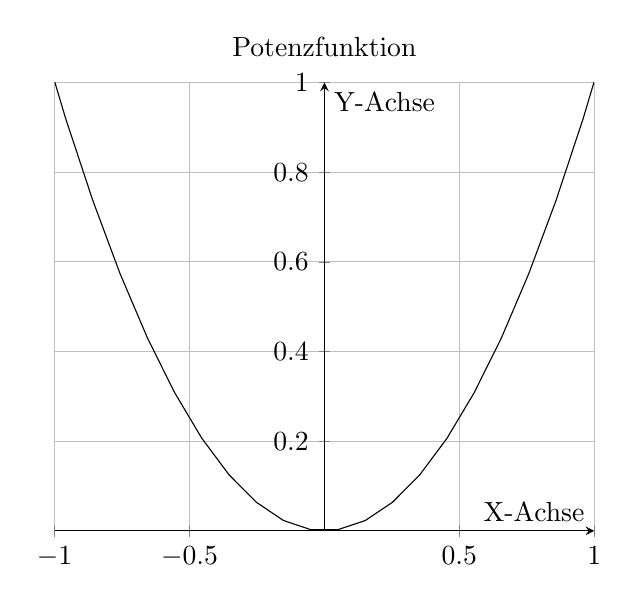
\begin{tikzpicture}
\begin{axis}[
    title={Potenzfunktion},
    xlabel={X-Achse},
    ylabel={Y-Achse},
    axis lines=middle, % Zentriert die Achsen
    xmin=-1, xmax=1, % Setzt die Grenzen für die X-Achse
    ymin=0, ymax=1, % Setzt die Grenzen für die Y-Achse
    grid=major, % Fügt ein Hauptgitter hinzu
]
\addplot[mark=none, samples=100] {x^2};
\end{axis}
\end{tikzpicture}
\caption{Quadratische Funktion mit $n>0$ und $ n\equiv0$ $(\mathrm{mod}2)$}
\end{figure}
\geogebra{https://www.geogebra.org/m/cand2jpf}
\subsubsection{Potenzfunktion mit $n>0$ und $ n\equiv1$ $(\mathrm{mod}2)$}
Ist $n>0$ und ungerade, so hat $f(x)=x^n$ die folgenden Eigenschaften.
\begin{itemize}
	\item $f(x)$ ist punktsymmetrisch zum Ursprung
	\item $f(x)$ verläuft von links nach rechts (vom 1. Quadranten zum 3. Quadranten), dies bedeutet die Form ist kubisch. %TODO Quadranten Blatt hinzufügen
	\item Je größer der Exponent ist, desto flacher verläuft $f$ für $-1<x<1$ und steiler für $x>1$ bzw. $x<-1$
	\item Die Funktion, die die geben Eigenschaften erfüllen sind alle monoton steigend
\end{itemize}
\begin{figure}[h]
\centering
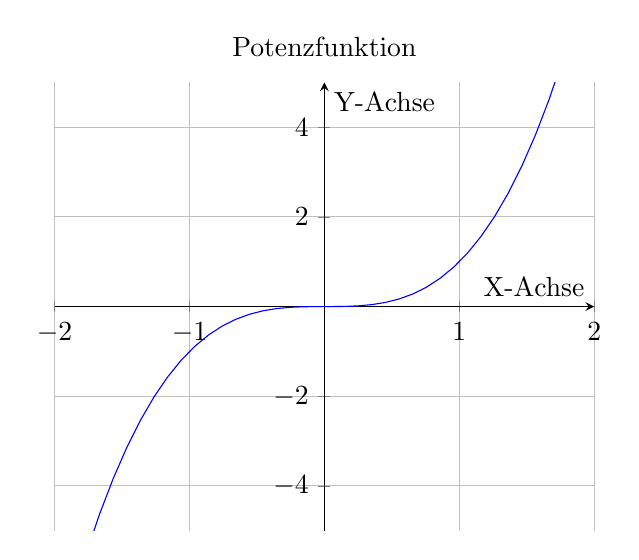
\begin{tikzpicture}
\begin{axis}[
    title={Potenzfunktion},
    xlabel={X-Achse},
    ylabel={Y-Achse},
    axis lines=middle, % Zentriert die Achsen
    xmin=-2, xmax=2, % Setzt die Grenzen für die X-Achse
    ymin=-5, ymax=5, % Setzt die Grenzen für die Y-Achse
    grid=major, % Fügt ein Hauptgitter hinzu
]
\addplot+[mark=none, samples=100]{x^3};
\end{axis}
\end{tikzpicture}
\caption{Potenzfunktion mit $n>0$ und $ n\equiv1$ $(\mathrm{mod}2)$}
\end{figure}
\pagebreak
\subsection{Potenzfunktion mit $n<0$ - Hyperbel}\label{sec:Potenzfunktionen/Potenzfunktionen mit negativem Exponenten}
Hat eine Funktion $f(x)=x^n$ einen negativen Exponenten, so bezeichnet man die Funktion als Hyperbel. Hyperbeln haben eine Definitionslücke, dass heißt, es gibt Zahlen, die man nicht für $x$ einsetzten darf. Hyperbeln verlaufen asymptotisch, dass heißt, es existieren Geraden, deren sich der Graph unendlich nah annähert, diese allerdings nicht tangiert. Besitzen sie einen geraden Exponenten verlaufen sie Achsensymmetrisch. Ist der Exponent ungerade, so verläuft der Graph punktsymmetrisch. 
\subsubsection{Potenzfunktionen mit $n<0$ und $n\equiv0(mod2)$}
Auch wie bei Potenzfunktionen mit einem positiven Exponenten gibt es Eigenschaften, die ein Graph einer Funktion mit einem negativen geraden Exponenten erfüllt.
\begin{itemize}
	\item Der Graph ist achsensymmetrisch
	\item Der Graph verläuft durch den Punkt $(-1;1)$
	\item Der Graph steigt für $x>0$ und fällt für $x<0$
\end{itemize}
\begin{figure}[h]
\centering
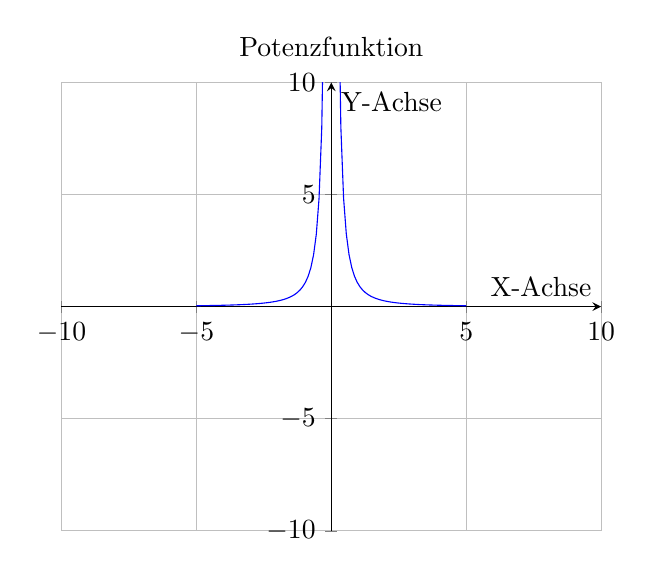
\begin{tikzpicture}
\begin{axis}[
    title={Potenzfunktion},
    xlabel={X-Achse},
    ylabel={Y-Achse},
    axis lines=middle, % Zentriert die Achsen
    xmin=-10, xmax=10, % Setzt die Grenzen für die X-Achse
    ymin=-10, ymax=10, % Setzt die Grenzen für die Y-Achse
    grid=major, % Fügt ein Hauptgitter hinzu
]
\addplot+[mark=none, samples=100]{x^(-2)};
\end{axis}
\end{tikzpicture}
\caption{Potenzfunktion mit $n<0$ und $ n\equiv0$ $(\mathrm{mod}2)$}
\end{figure}
\subsubsection{Potenzfunktionen mit $n<0$ und $n\equiv1(mod2)$}
Die Eigenschaften einer Potenzfunktion mit einem negativen ungeraden Exponenten sind die folgenden. 
\begin{itemize}
	\item Der Graph ist punktsymmetrisch zum Ursprung
	\item Der Graph verläuft durch den Punkt $(-1;1)$
	\item Der Graph fällt für $x>1$ sowohl als auch für $x<0$
\end{itemize}
\begin{figure}[h]
\centering
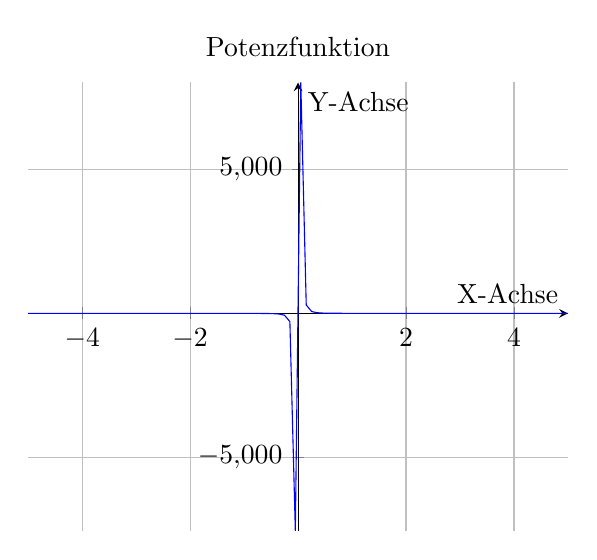
\begin{tikzpicture}
\begin{axis}[
    title={Potenzfunktion},
    xlabel={X-Achse},
    ylabel={Y-Achse},
    axis lines=middle, % Zentriert die Achsen
    grid=major, % Fügt ein Hauptgitter hinzu
]
\addplot+[mark=none, samples=100]{x^(-3)};
\end{axis}
\end{tikzpicture}
\caption{Potenzfunktion mit $n<0$ und $ n\equiv0$ $(\mathrm{mod}2)$}
\end{figure}
\pagebreak
\subsection{Ausbildung des Graphen bei Potenzfunktion}\label{sec:Potenzfunktionen/Ausbildung des Graphen bei Potenzfunktionen}
Ähnlich wie bei linearen Funktion stellt eine Potenzfunktion ein Verhältnis von einem $y$-Wert zu einem $y$-Wert dar. Durch die Multiplikation bei einer Potenzfunktion, die durch den Exponenten bestimmt wird, kann beim Einsetzten in eine Varibale, die einen geraden Exponenten besitzt keine negative Zahl als Ergebnis entstehen. Bei einem ungeraden Exponenten kann wiederum eine negative Zahle als Ergebnis einer Multiplikation entstehen. Bei einer kubisch verlaufenden Potenzfunktion ist es wichtig, zu wissen, dass ein Exponenten angibt, wie oft eine Zahl mit sich selbst multipliziert wird. Kubisch verlaufende Funktionen sind Funktionen, die einen ungeraden Exponenten besitzen. Weil in der Variable $x$ jede Zahl von positiv bis negativ enthalten ist und das Multiplizieren von einer ungeraden Anzahl an Faktoren bei einer negativen Basis ein negatives Ergebnis ergibt, prägt sich der Graph in der kubischen Form aus. Da das Multipliziert von einer ungeraden Anzahl an positiven Faktoren ein positives Ergebnis ergibt, steigt der Graph im 2. Quadranten. 




% Polynome
\section{Polynome}
% Differenzenquotient und Mittlereaenderungsrate und Sekante
\input{Kapitel/Differenzenquotient_Mittlereaenderungsrate_Sekante/Differenzenquotient_Mittlereaenderungsrate_Sekante.tex}
% Momentane Änderungsrate
\section{Momentane Änderungsrate}
% Ableitung
\input{Kapitel/Ableitung/Ableitung.tex}
% Potenzgesetze
\section{Potenzgesetzte}
% Extrempunkte algebraisch bestimmen
\input{Kapitel/Extrempunkte_algebraisch_berechnen/Extrempunkte_algebraisch_berechnen.tex}
\section{Tangenten}
% Integral
\input{Kapitel/Integrale/Integrale.tex}
%% Trigonometrie
\section{Trigonometrie}
	\subsection{Geometrische Trigonometrie}
	Das Thema Trigonometrie in der Geometrie umfasst eine Reihe an verschiedenen Unterthemen. Hierbei
spielt das rechtwinkelige Dreieck eine wesentliche Rolle und bestimmt somit auch die Wurzeln der
Trigonometrie. Bei der geometrischen Trigonometrie geht es vorwiegend um das Bestimmen von
Seitenlängen oder Winkeln.
\begin{center}
	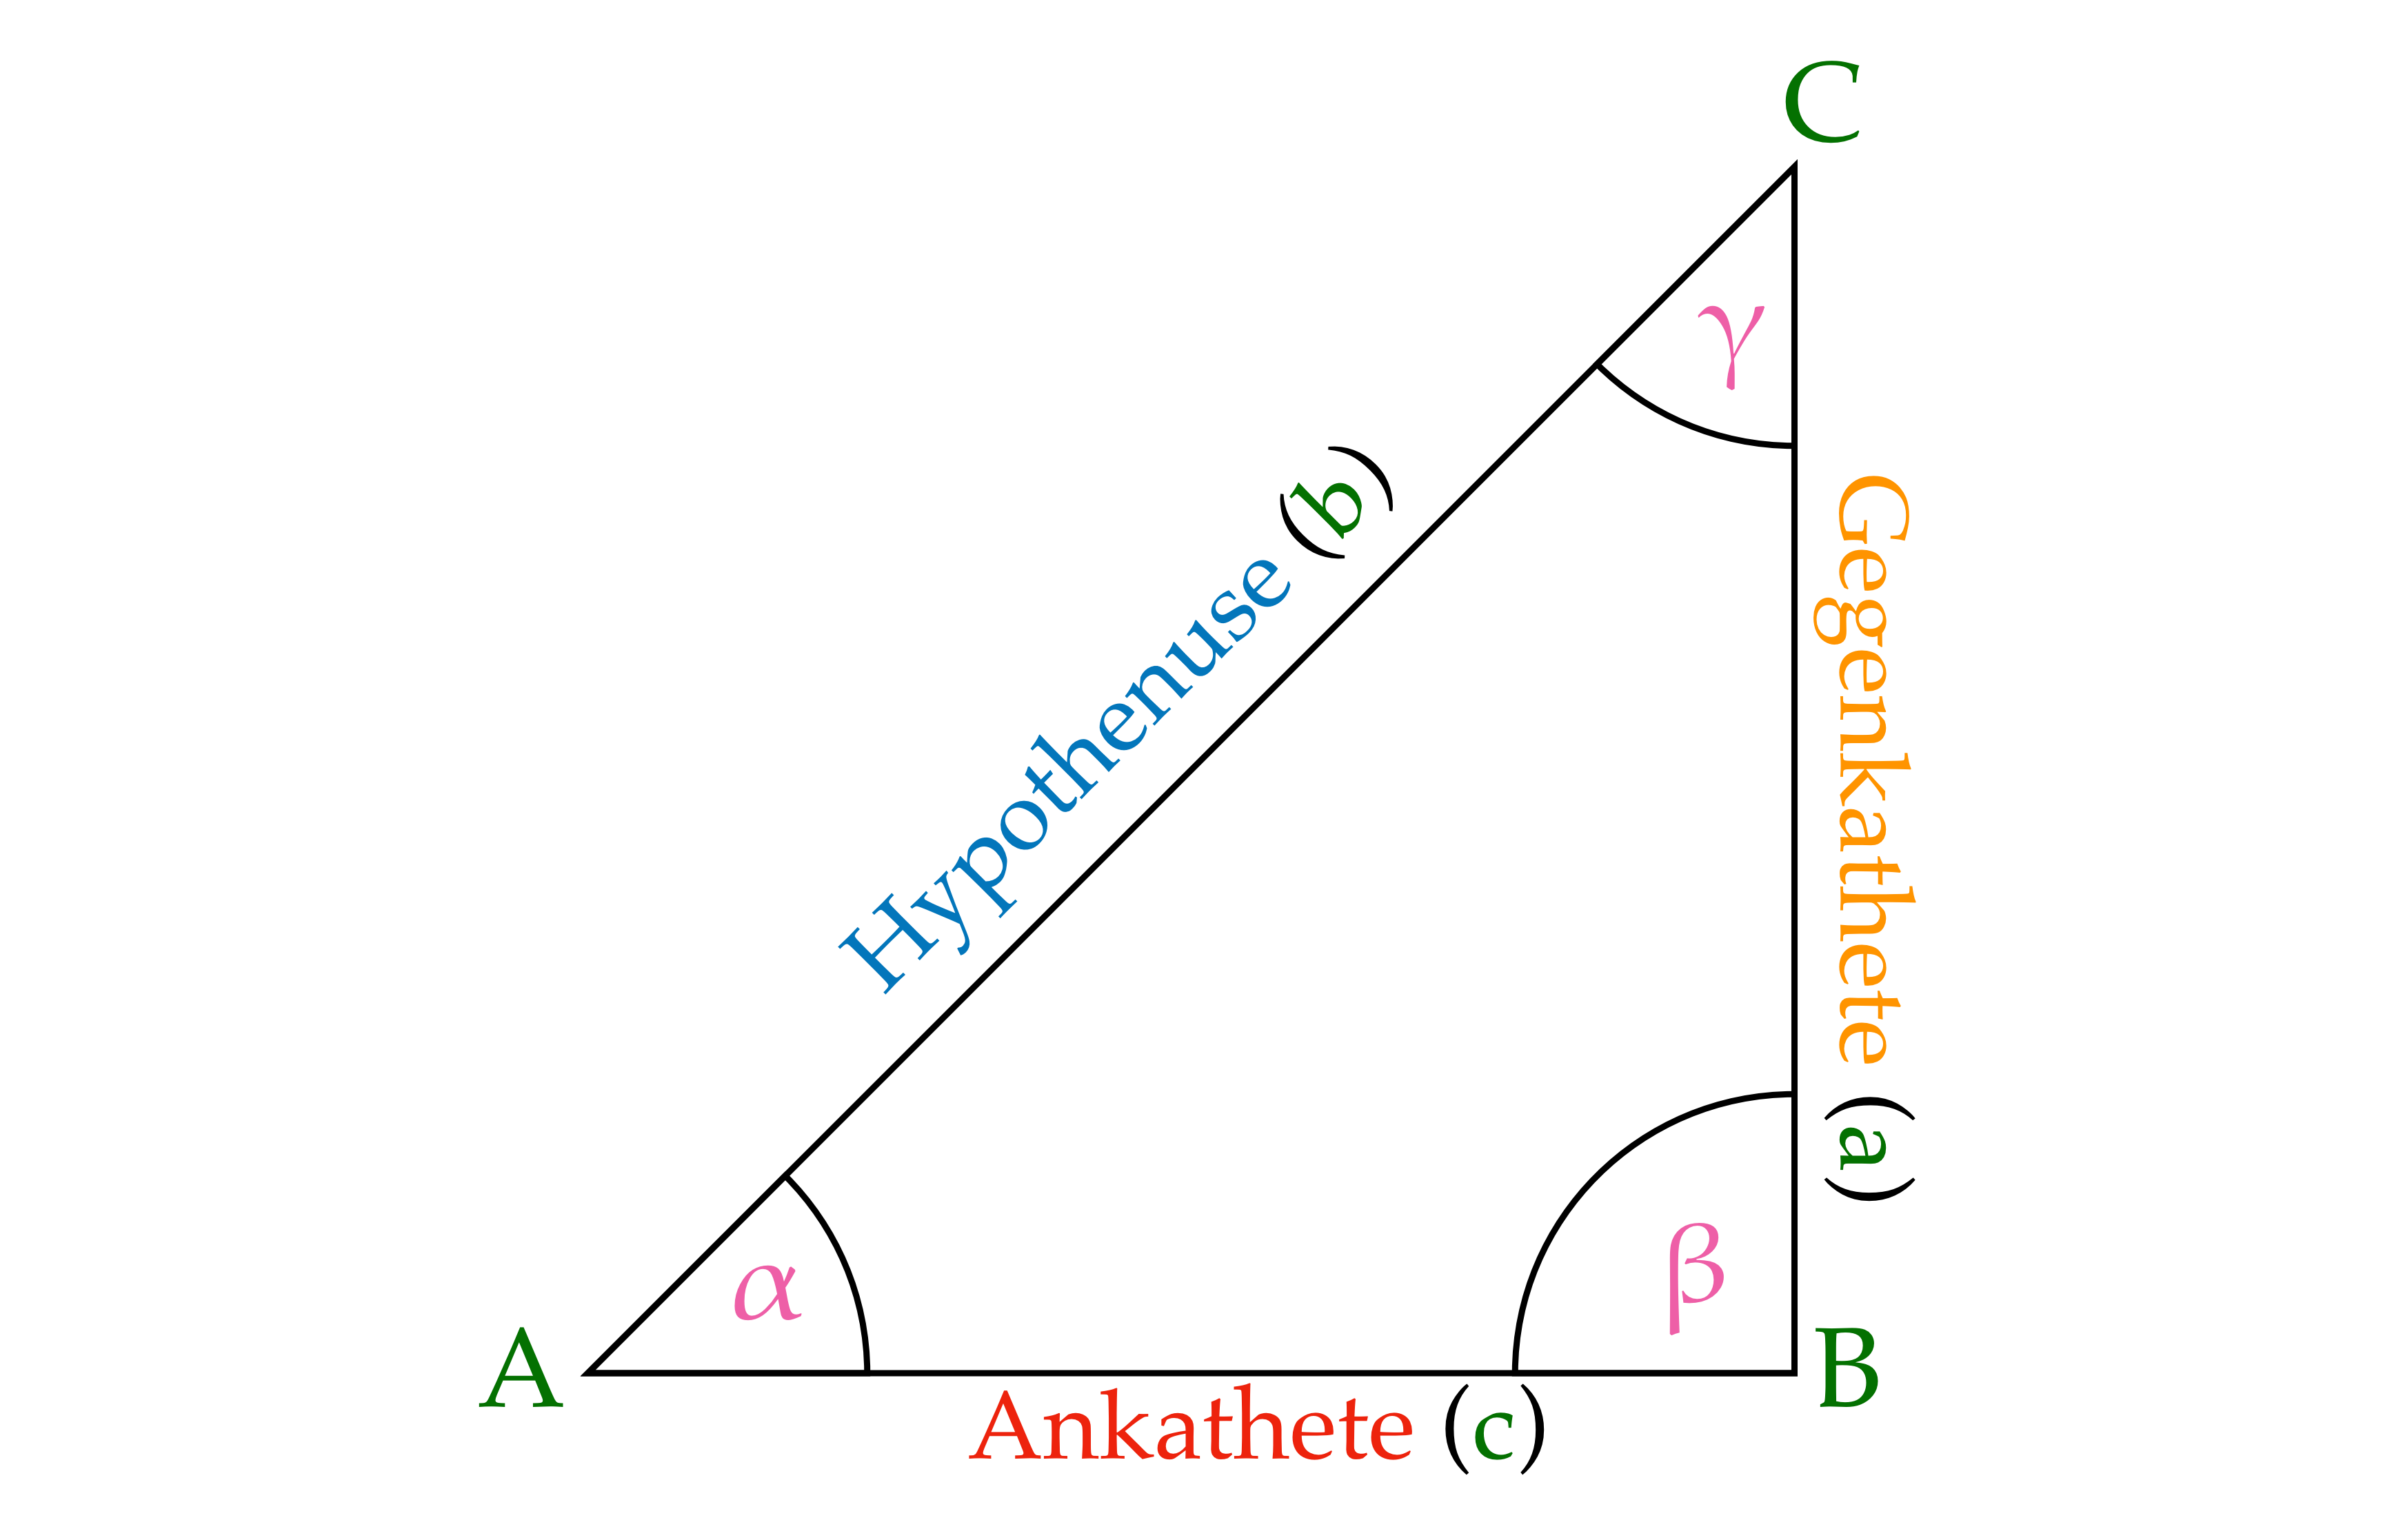
\includegraphics[width=200pt, height=130pt]{Media/Dreieck}
\end{center}
\begin{itemize}
	\item[\textcolor{darkgreen}{\textbf{A, B, C}}]{}
	Die Ecken eines rechtwinkeligen Dreiecks sind mit großen Buchstaben gekennzeichnet
	
	\item[\textcolor{darkgreen}{\textbf{a,b,c}}]{Die gegenüberliegenden Seiten sind mit dem jeweils
	gleichen Buchstab in klein gekennzeichnet
	Stellen jeweils die Winkel zwischen den anliegenden Seiten dar und ergeben zusammen 180 Grad.
	Die Gegenkathete stellt die Höhe
	des Dreiecks dar, während die Ankathete die Seite ist, die am rechten Winkel  und  anliegt}
	
	
	\item[\textcolor{blue}{\textbf{Hypothenuse}}]{}
	Die Hypothenuse stellt im Dreieck die Seite $b$ dar. Sie ist die längste Seite und immer
	gegenübervon rechten Winkel, wobei sie nie an ihm anliegt. 


	\item[\textcolor{red}{\textbf{Ankathete}}]{}
	Die Ankathete ist die Seite $c$ in einem Dreieck und liegt immer am rechten Winkel an. Sie bildet mit der Gegenkathete den rechten Winkel und ist hierbei immer kürzer als die Hypothenuse
	
	
	\item[\textcolor{orange}{\textbf{Gegenkathete}}]{}
	Die Gegenkathete beschreibt in einem Dreieck die Seite a und liegt direkt an dem rechten Winkel,
	den sie mit der Ankathete bildet. 
\end{itemize}
\pagebreak

% Neue Seite ################################################################################################################################################
\subsection{Berechnung der Seiten und des Winkels}
	Um eine Berechnung der Seiten durchführen zu können, muss verwendet man folgende Formeln:\\
	\\
	
\textbf{Sinus} \[ \sin(\alpha)=\frac{Gegenkathete}{Hypotenuse} \]
\textbf{Cosinus} \[ \cos(\alpha)=\frac{Ankathete}{Hypothenuse} \]
\textbf{Tangens} \[ \tan(\alpha)=\frac{Gegenkathete}{Ankathete} \]
\\
\\
Um einen ersten Anhaltspunkt zu schaffen, kann man sich an dem folgenden Algorythmus orientieren. 

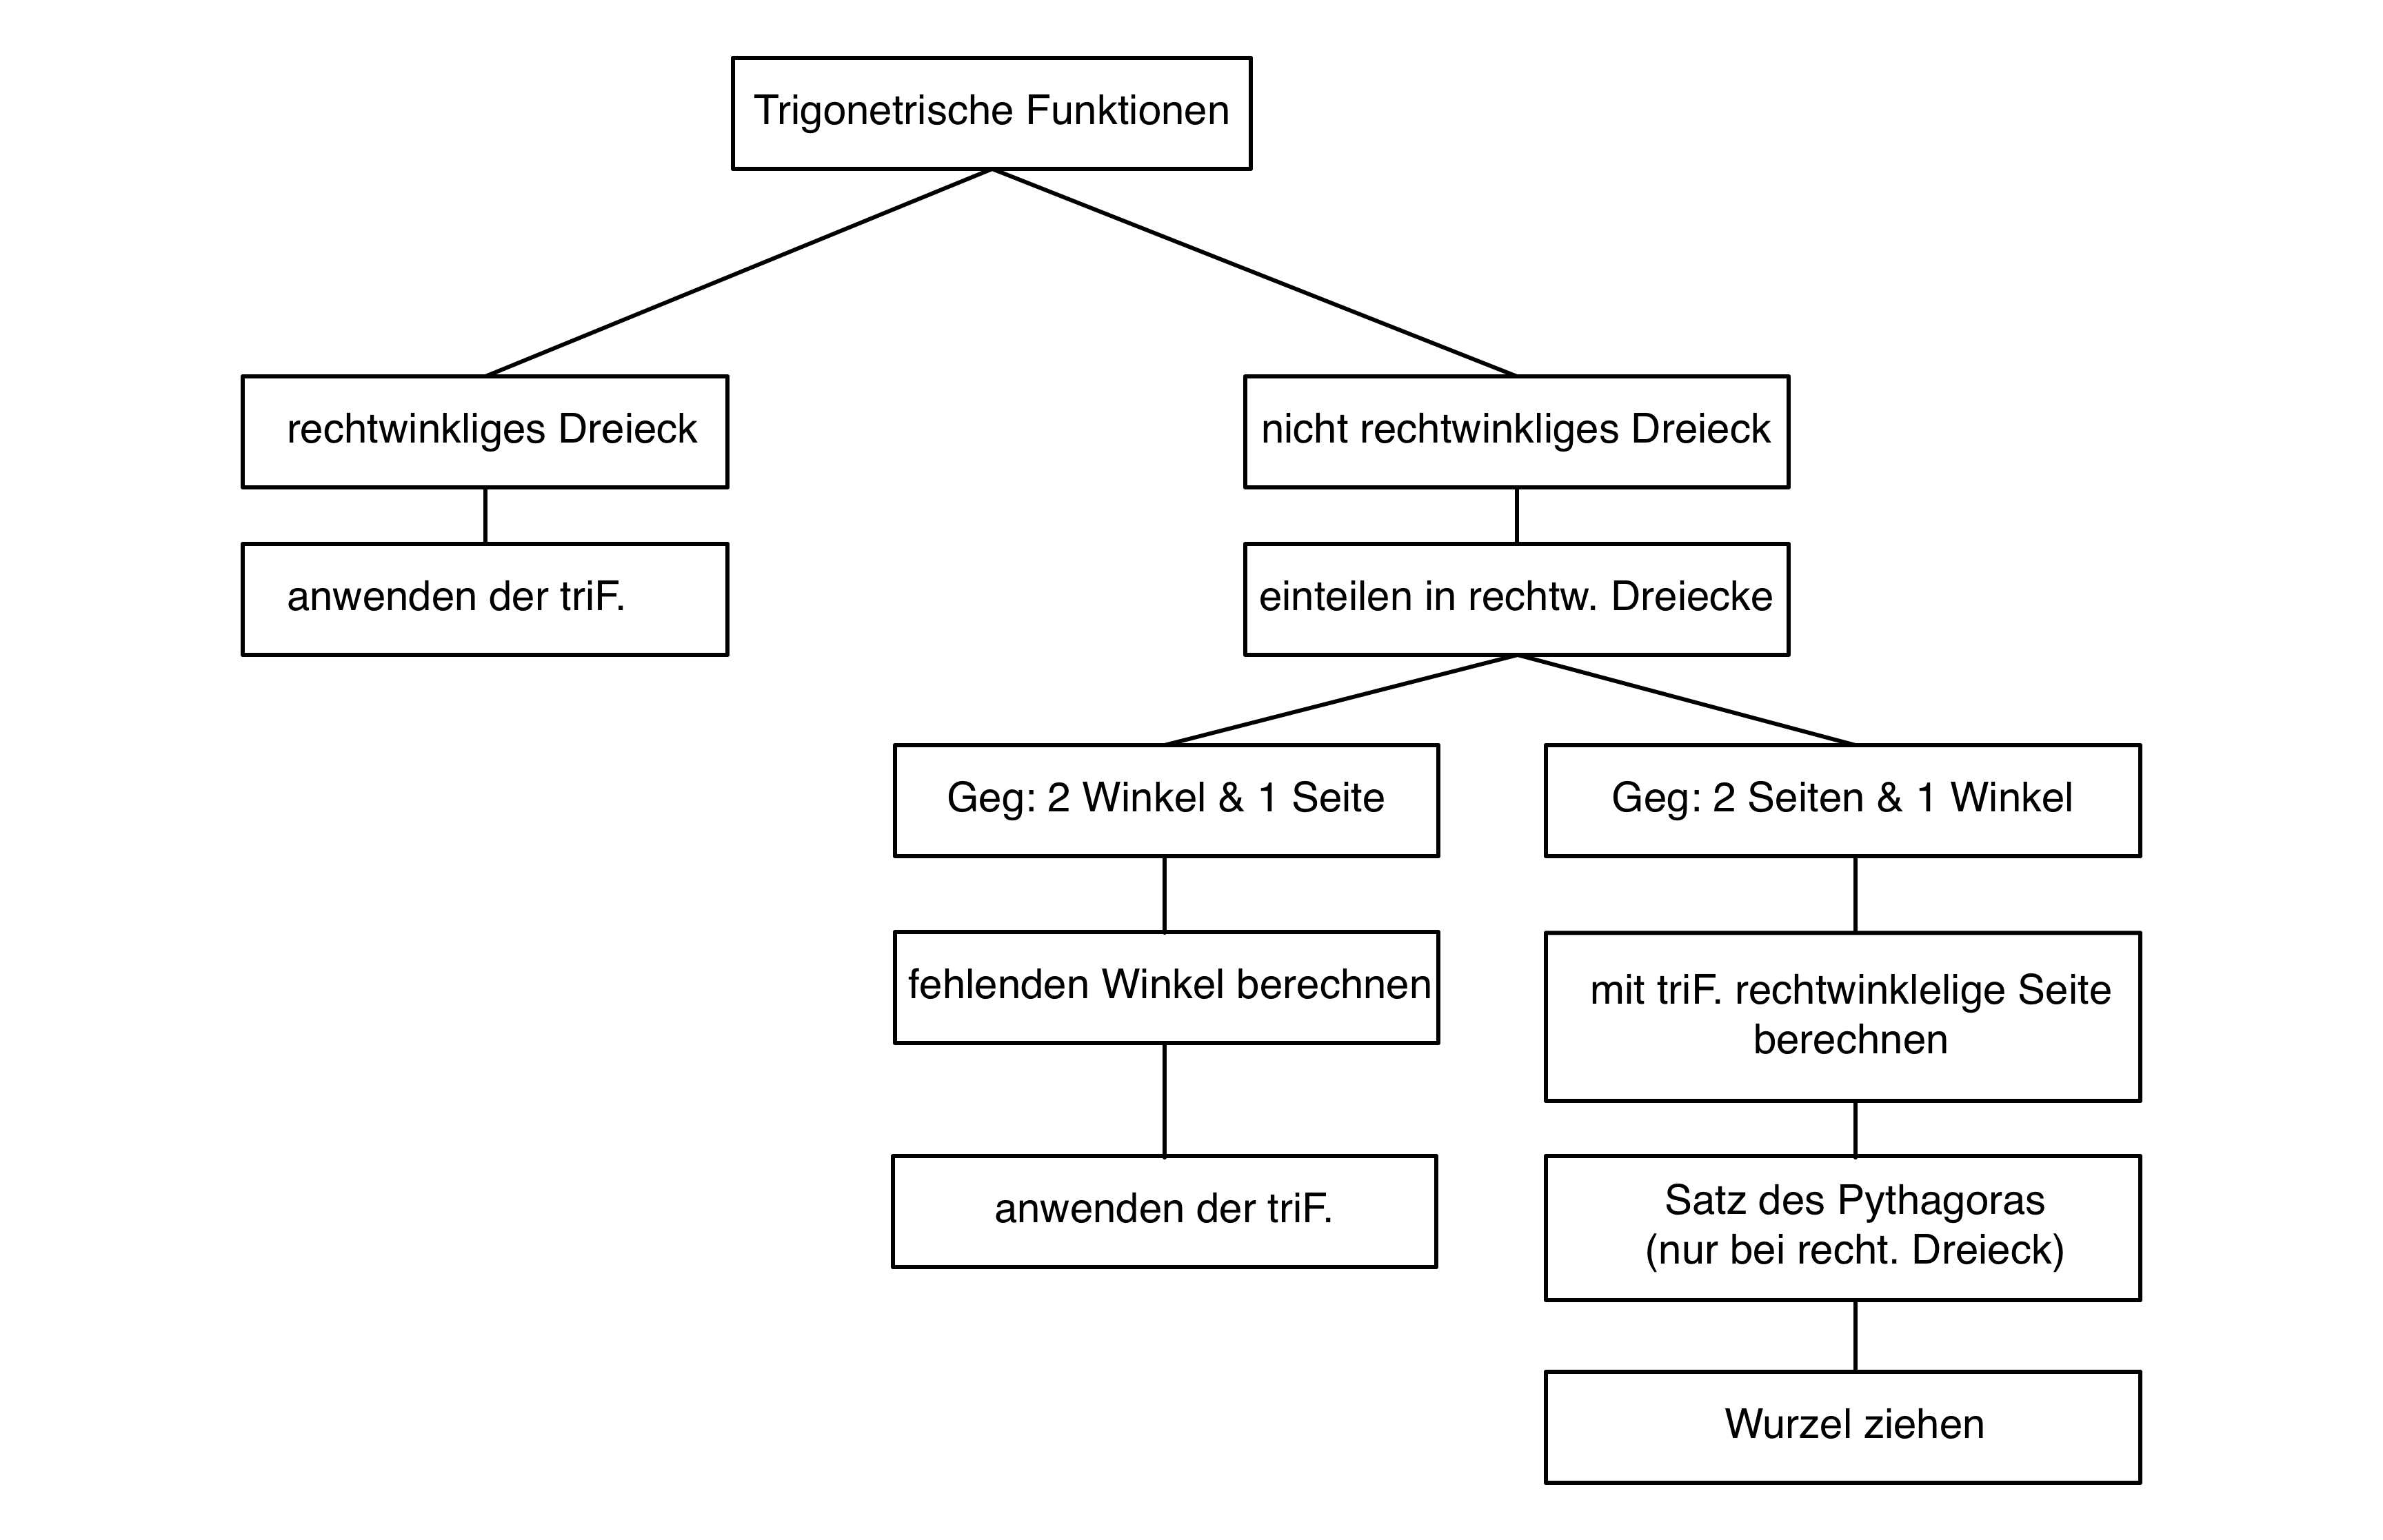
\includegraphics[width=15cm]{Media/Algorythmus_Berechnung_eines_Dreiecks}



\pagebreak
% Neue Seite ################################################################################################################################################

\subsection{Trigonometrische Funktionen}
 	Auch in der Analyses spielt die Trigonometrie einen wichtige Rolle. Sie ermöglicht es periodische Prozesse darzustellen und mit ihnen zu rechnen. So lassen sich Sinus, Cosinus und Tangens jeweils im Koordinatensystem herleiten am Einheitskreis.

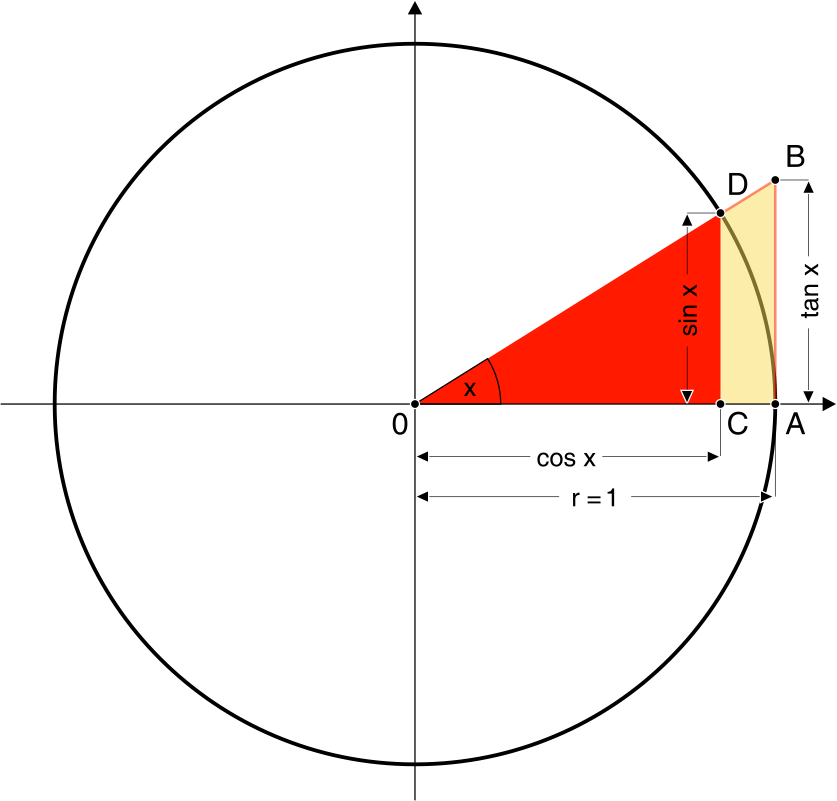
\includegraphics[width=10cm]{Media/Winkelfunktionen_Einheitskreis}\\
So stellt Sinus die Höhe der Gegenkathete in Abhängigkeit von dem Bogenmass, welches mit Hilfe des
Winkels Alpha berechnet wird. Cosinus hingegen stellt die Ankathete in Abhängigkeit des Bogenmasses dar. Hierbei orientieren sich die Eckpunkt jeweils an dem Einheitskreis und laufen auf 
diesem gegen den Uhrzeigersinn. Hierdurch entsteht die wellenförmige Ausprägung des Graphen. Da Sinus die Höhe der Gegenkathete darstellt in Abhängigkeit von dem Bogenmass befindet sich die
dargestellte Höhe der Gegenkathete auf einer Höhe von $\pi$ auf der X-Achse. 
\\
\\
\textbf{Begründung der Periodenlänge}
Durch den Einheitskreis wird die Perioden länge bestimmt, da das Bogenmass auf der X-Achse dargestellt wird. So ist eine halbe Umrundung des Kreises genau ein $\pi$ lang. 


\subsection{Überleitung zu trigonmetrische Funktionen}
Aufgrund der Veränderung der verschiedenen Seitenlängen des rechtwinkeligen Dreiecks, welche durch die jeweilge trigonometrische Funktion dargestellt wird und abhängi
von dem Winkel $\alpha$ ist, entsteht die pregnante Form von Sinus und Cosinus. 
\\
%\link{https://de.wikipedia.org/wiki/Trigonometrische_Funktion#/media/Datei:Circle_cos_sin.gif}{Veranschaulichung Entstehung von Sinus Cosinus}


\subsection{Normalform einer trigonometrischen Funktion}
Ähnlich wie quadratische Funktionen oder lineare Funktionen gibt es ebenfalls einen Normalform der Sinus Funktion.
\[a\cdot sin(b(x+d))+e\]
\\
$a$: Streckfaktor auf der X-Achse(Amplitude) \\
$b$: Streckfaktor auf der Y-Achse (Periodenlänge)\\
$d$: Verschiebung auf der X-Achse\\
$e$: Verschiebung auf der Y-Achse \\
	\pagebreak
	
% Neue Seite ################################################################################################################################################
\subsection{Moddelierung der Sinus Funktion}
Für die Moddelierung einer Sinus oder Cosinus Funktion kann man wie folgt vorgehen.

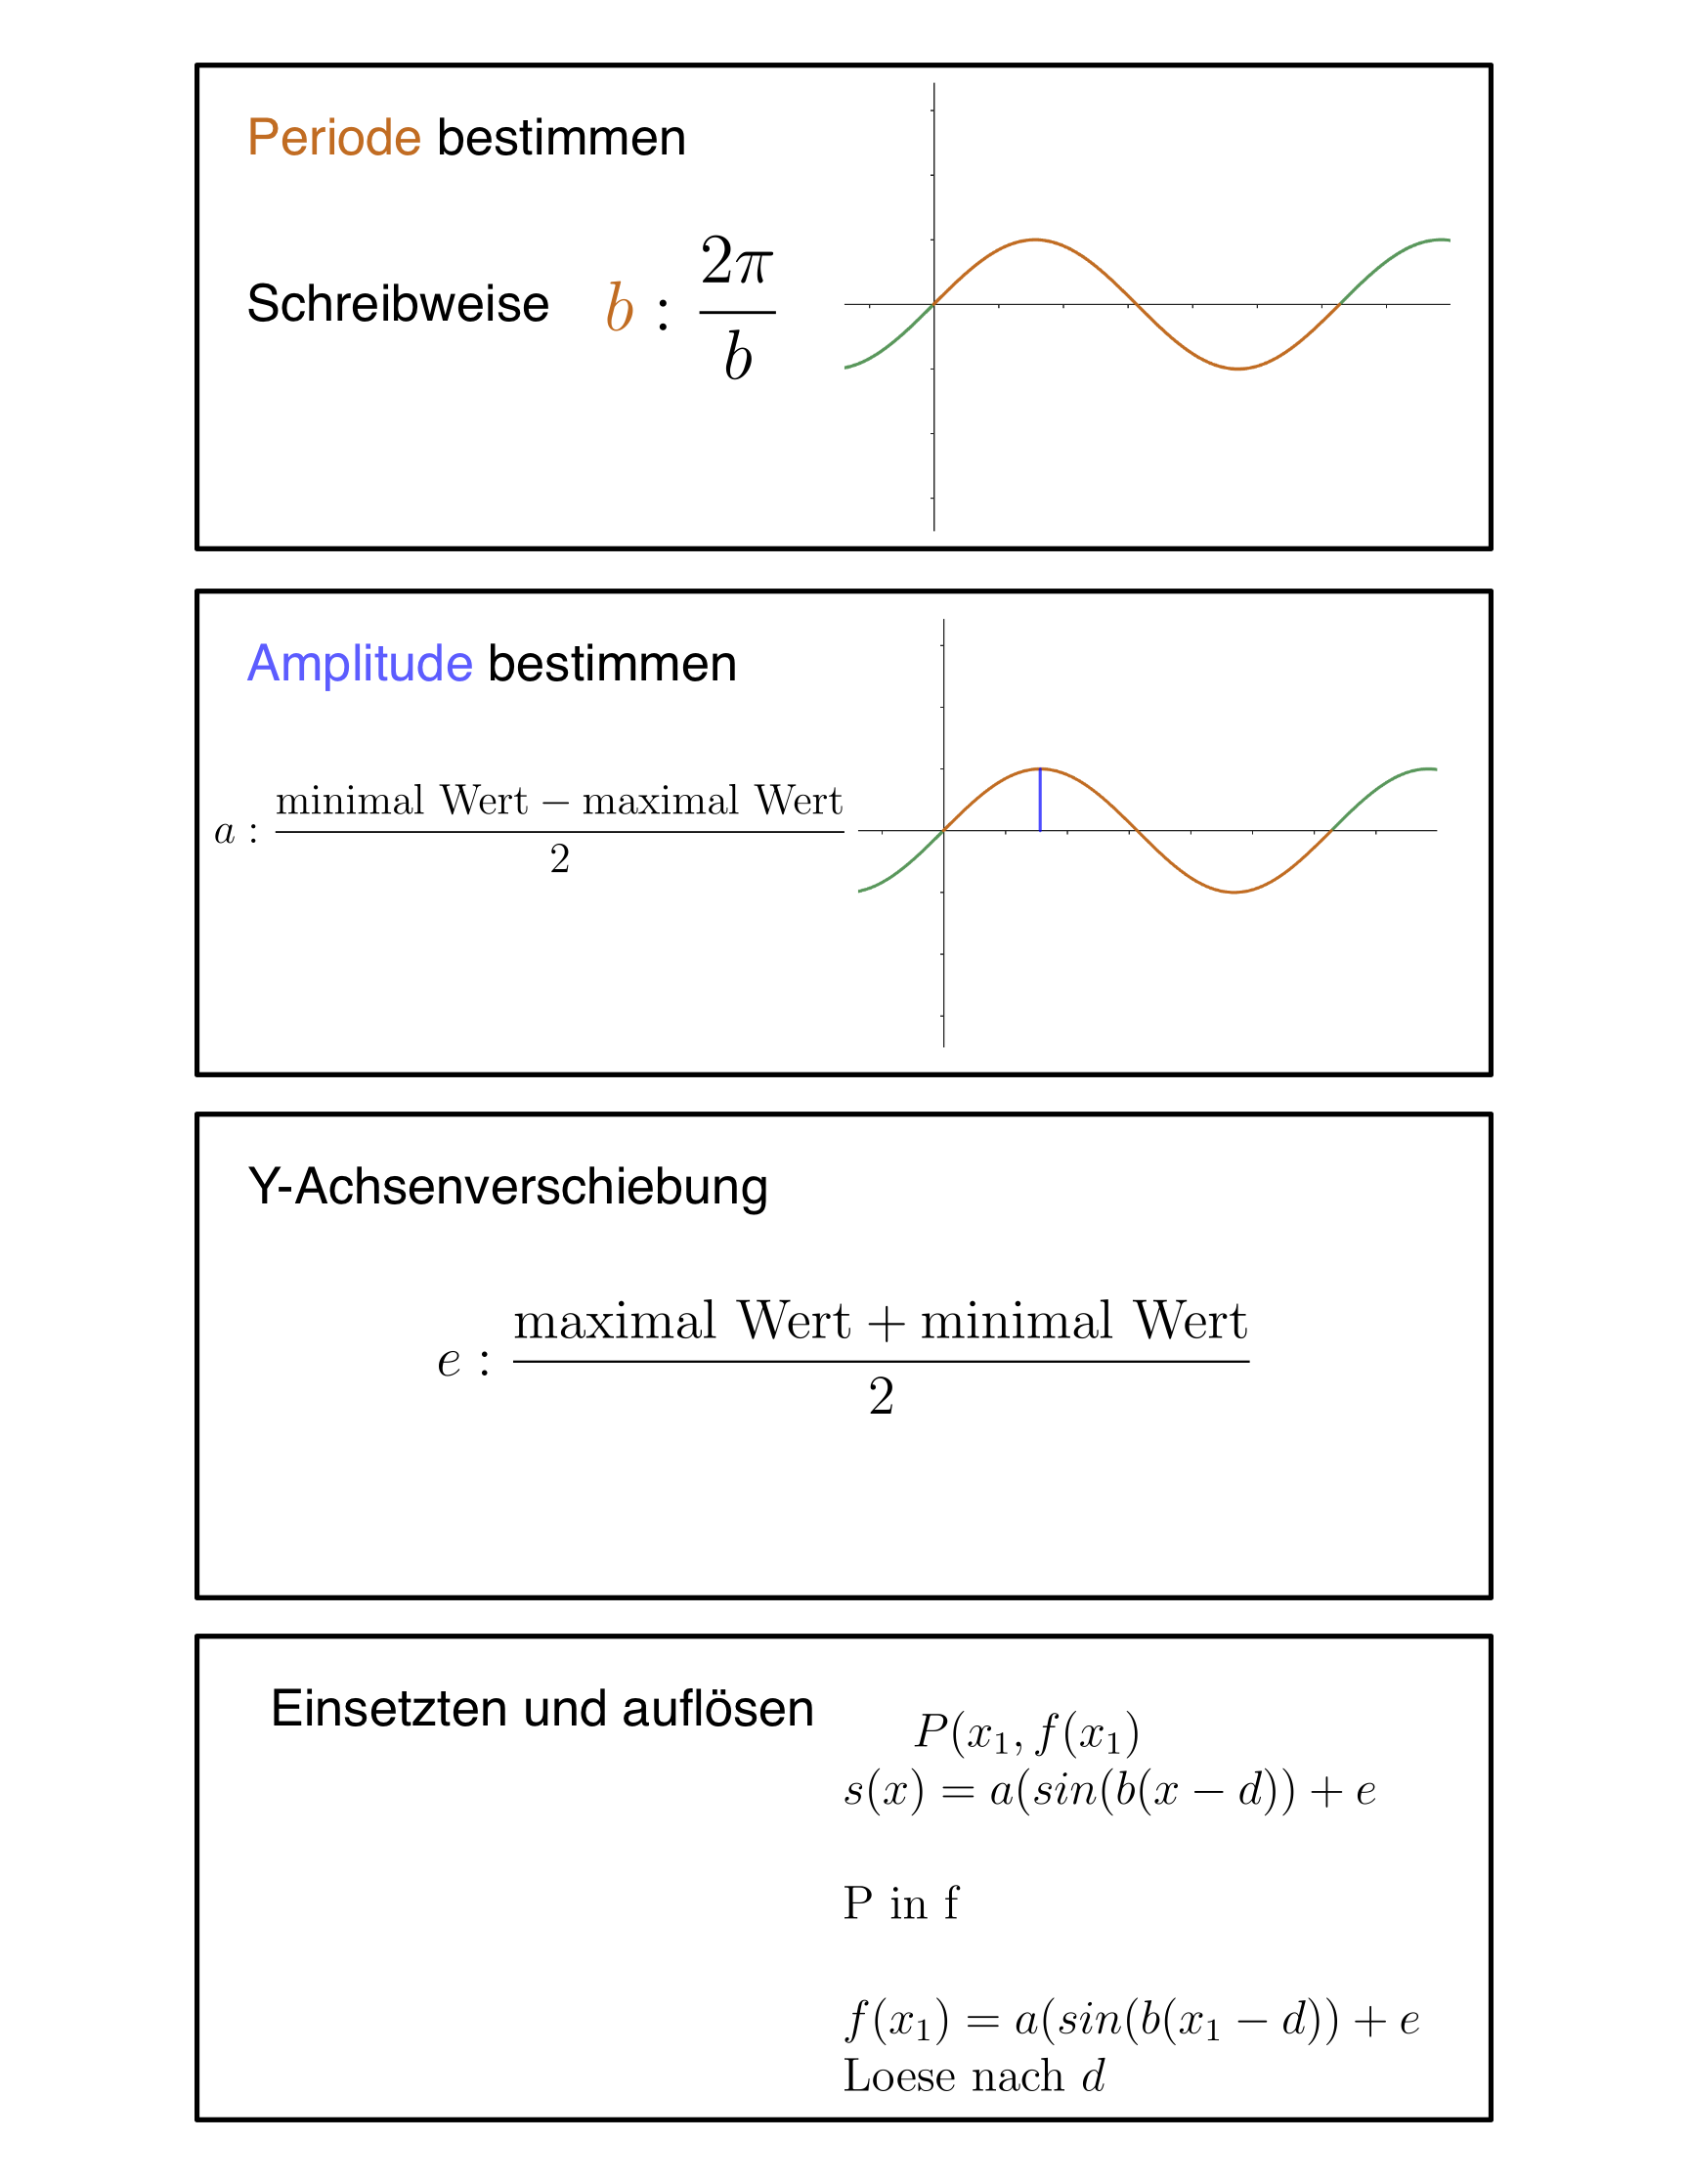
\includegraphics[width=13cm]{Media/Modelierung_von_Sinus_Algorythmus}


% Exponentialfunktionen
\section{Exponentialfunktionen}\label{sec:Exponentialfunktionen}
Eine Exponentialfunktion stellt einen exponentiell Verlauf eines Graphen dar. 
\begin{figure}[h!]
\centering
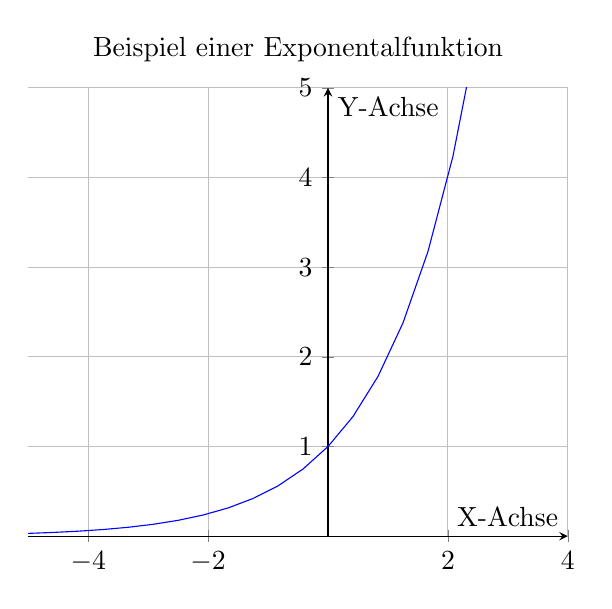
\begin{tikzpicture}
\begin{axis}[
    title={Beispiel einer Exponentalfunktion},
    xlabel={X-Achse},
    ylabel={Y-Achse},
    axis lines=middle, % Zentriert die Achsen
    xmin=-5, xmax=4, % Setzt die Grenzen für die X-Achse
    ymin=0, ymax=5, % Setzt die Grenzen für die Y-Achse
    grid=major, % Fügt ein Hauptgitter hinzu
]
% Hier fügen Sie Ihre Daten ein
\addplot+[mark=none] {2^x};
\end{axis}
\end{tikzpicture}
\caption{Funktionsgraph von $f(x)=2^x$}
\end{figure}

\subsection{Normalform}\label{sec:Exponentialfunktionen/Normalform}

Hierbei folgt einer Exponentialfunktion der folgenden Form: 
\[f(x)=a\cdot b^x\] Wobei $b>0 \land b\neq 0  $   sein muss.\\
 $a$ wird hierbei als Startwert bezeichnet. Innermathematisch spricht man von $a$ als Streckfaktor und von $b$ als Wachstumsfaktor. \\
 
 \subsubsection{Faktor \mbox{\boldmath$a$}  - Startwert} 
 Der Koeffizent $a$ stellt bei einer exponentiell verlaufenden Funktion den Startwert dar und zugleich auch Streckfaktor der Funktion. Er wird für jedes $x$ immer mit der Basis $b$ multipliziert. 
  \paragraph{Beispiel} sei sei $-0.5\le b\ge 2 $ und $-1\le a\ge 1$ für $f(x)=ab^x$
  \begin{align*} 
a&:-1			& a&:	0				&. a&: 1\\
x&:-1           &  x &: 0              &  x &:1\\
b&:-0.5			& b&:-0.5					& b&:-0.5\\
\\
f(-1)&=(-1)\cdot(-0.5)^{-1}	& f(0)&=0\cdot0.5^0	& f(1)&=1\cdot(-0.5)^1\\  
&= 2 & &=0 & &=-0.5\\
\end{align*}


  \subsubsection{Basis \mbox{\boldmath$b$} - Wachstumsfaktor } Die Basis $b$ ist hierbei von großer Bedeutung, da diese mit dem $x$ für jedes $x$ multipliziert wird. Da bei exponentiell Verläufen schnell das Vielfache der Basis erreicht wird, braucht der Wert von $b$ nur sehr gering sein, um eine große Auswirkung zu haben. Ebenfalls hat $b$ eine große Auswirkung den Verlauf in Bezug auf den Schnittpunkt mit der Y-Achse. $b$ ist hauptverantwortlich für diese, da durch $x$ die Anzahl der Multiplikationen mit sich selbst bestimmt wird. 


\paragraph{Beispiel} sei $-0.5\le b\ge 2 $ und $-1\le x\ge 2$ für $f(x)=b^x$
   	
\begin{align*} 
x&:-1           &  x &: 0              &  x &:1\\
b&:-0.5			& b&:-0.5					& b&:-0.5\\
f(-1)&=-0.5^{-1}	& f(0)&=a-0.5^0	& f(1)&=-0.5^1\\  
&= -2 & &=1 & &=-0.5
\end{align*}

\begin{align*}
x&:-1           &  x &: 0              &  x &:1\\
b&:0			& b&:0					& b&:0\\
f(-1)&=0^{-1}	& f(0)&=0^0	& f(1)&=0^1\\  
&= \infty & &=1 & &=0
\end{align*}

\begin{align*}
x&:-1           &  x &: 0              &  x &:1\\
b&:1			& b&:1					& b&:1\\
f(-1)&=1^{-1}	& f(0)&=1^0	& f(1)&=1^1\\  
&=1  & &=1 & &=1
\end{align*}

\begin{align*}
x&:-1           &  x &: 0              &  x &:1\\
b&:2			& b&:2					& b&:2\\
f(-1)&=2^{-1}	& f(0)&=2^0	& f(1)&=2^1\\  
&=0.5  & &=1 & &=2
\end{align*}
An dem Beispiel kann man sehen, dass egal welche Zahl die Basis $b$ annimmt es beim Einsetzten von
$0$ für $x$ immer zu $1$ kommt. Auffällig ist hierbei, dass setzt man für $b : 1$ ein, so erhält man zu jedem $x$ immer den Wert $1$. Dies ist die Begründung für die Schnittstelle mit der Y-Achse bei $1$, wenn $a=1$ ist. Setzt man nun für $b$ einen Wert ein, der größer als 1 ist, so verändert sich etwas. Die Basis $b$ wird für $x$ mit sich selber multipliziert. Nimmt $b$ nun einen Wert von $1.01$ an, so wird wie folgt für $x=3$ gerechnet. 
	\[\underbrace{1.01}_{1}\cdot\underbrace{1.01}_{2}\cdot\underbrace{1.01}_{3}\]
	\[=1.030301\]
	Die Differenz zwischen $1$ und $b$ wird vervielfacht. Alleine diese kleine Differenz reicht aus, um eine deutliche Ausprägung zu verursachen in dem Graphen von $f(x)$.
	
	
 
 %TODO Hier muss ein Beispiel kommen, warum sich b immer gleich auswirkt auf den Verlauf des Graphen. Auch ein Rechenbeispiel, welches zeigt, warum es dort eine Schnittstelle gibt und warum die prozentuale Steigung ensteht. 

 

 
 \subsection{Prozentuale Zunahme}\label{sec:Exponentialfunktionen/Prozentuale Zunahme}
 Einen exponentiellen Verlauf kann man unteranderem an einer prozentualen Veränderung erkennen. So lässt sich sagen, dass sei $b>1$ eine prozentuale Steigung der Differenz zwischen
 $1$ und dem Wert, den $b$ annimmt bestimmen. \\
 Nimmt man an, dass sei $b=1.01$, so ist $0.1$ gleich $1\%$ von $1$ und besitzt somit eine prozentuale Zunahme von $1\%$. Übertragt man diesen Sachverhalt auf eine weitere Basis,
 welche $b>1$ erfüllt, so lässt sich ebenfalls der Übertrag als prozentuale Steigung definieren.
\paragraph{Beispiel} Sei \ $ b \in\{x : x \in \mathbb{R}, x > 1\}$ \
\[f(x)=1.04^x\Rightarrow4\%\]
So folgt aus $b=1.04$, dass eine Zunahme von $4\%$ vorliegt.\\
\\
\[f(x)=1.5^x\Rightarrow50\%\]
So folgt aus $b=1.5$, dass eine Zunahme von $50\%$ vorliegt.\\
\\
\[f(x)=1.9^x\Rightarrow90\%\]
So folgt aus $b=1.9$, dass eine Zunahme von $90\%$ vorliegt.\\
\\
\[f(x)=2.6^x\Rightarrow\ 160\%\]
So folgt aus $b=2.6$, dass eine Zunahme von $160\%$ vorliegt, da sich eine prozentuale Zunahme nur für die Differenz zwischen $b$ und $b=1$ ausprägt.\\
\\
\[f(x)=0.8^x\Rightarrow20\%\]
So folgt aus $b=0.8$, dass eine Abnahme von $20\%$ vorliegt. Zu dieser Annahme kommt man, indem man sich überlegt, dass $b=1=100\%$ sind. Hat man nun nur $b=0.8$ anstelle von $b=1$ , so ergibt sich hieraus die Verringerung von $20\%$
\pagebreak
\subsection{Prozentuale Zunahme/Abnahme algorithmisch bestimmen}\label{sec:Exponentialfunktionen/Prozentuale Zunahme/Abnahme algorithmisch bestimmen}
Um die Berechnung der prozentualen Änderung des Graphen zu bestimmen kann man algorythmisch vorgehen.
\begin{center}	
\tikzstyle{prozentuelleZunahme} = [rectangle, rounded corners, minimum width=3cm, minimum height=1cm, text centered, font=\normalsize, color=black, draw=f3551e38-74df-57e2-b793-83d7fe876c85, line width=1, fill=white]
\tikzstyle{Entscheidung} = [diamond, minimum width=3cm, minimum height=2cm, text centered, font=\normalsize, color=black, draw=f3551e38-74df-57e2-b793-83d7fe876c85, line width=1, fill=white]
\tikzstyle{Prozessbox} = [rectangle, minimum width=3cm, minimum height=1cm, text centered, font=\normalsize, color=black, draw=f3551e38-74df-57e2-b793-83d7fe876c85, line width=1, fill=white]
\tikzstyle{linie} = [thick, line width=1, ->, >=stealth]
\begin{tikzpicture}[node distance=2cm]
\node (ProzessBoxing) [prozentuelleZunahme] {Prozentuelle Zunahme};
\node (pfeil1) [Entscheidung, below of=ProzessBoxing, yshift=-0.5cm] {$b>1$};
\node (pfeil2) [Prozessbox, below of=pfeil1, yshift=-0.5cm,xshift=-3cm] {$b-1$};
\node (pfeil3) [Prozessbox, right of=pfeil2, xshift=4cm] {$1-b$};
\node (pfeil4) [Prozessbox, below of=pfeil2] {$\cdot100$};
\node (pfeil5) [Prozessbox, right of=pfeil4, xshift=4cm] {$\cdot100$};
\draw [linie] (ProzessBoxing) --  (pfeil1);
\draw [linie] (pfeil1) -| node[anchor=south] {ja} (pfeil2);
\draw [linie] (pfeil1) -| node[anchor=south] {nein} (pfeil3);
\draw [linie] (pfeil3) --  (pfeil5);
\draw [linie] (pfeil2) --  (pfeil4);
\end{tikzpicture}
\end{center}
\pagebreak
\subsection{Umformung von der normalen Exponentialfunktion zu der E-Funktion}
Da sich die $e$-Funktion besonders gut differenzieren und integrieren lässt, nutzt man diese, um Sachverhalte darzustellen. Hierfür formt man die normale Exponentialfunktion so um, dass man sie als $e$-Funktion schreiben kann. Hierfür ist es relevant die Bedeutung der folgenden Normalform zu kennen. 
\subsubsection{Normalform}
\begin{align*}
	f(x)=a\cdot e^{k\cdot x+d}+c
\end{align*}
\geogebra{https://www.geogebra.org/m/bkar24wm}

\subsubsection{$a$ - Streckfaktor}
Der Faktor $a$ ist bestimmt die Streckungs/Stauchungs des Graphen. Wird dieser negativ, so wird der Graph an der $X$-Achse gespiegelt. Der Grund hierfür ist, dass ist $a$ negativ, werden die gesamten Werte des Graphen ebenfalls negativ. 
%ToDo Hier fehlt ein Graph mit einem Vergleich
\begin{figure}[h!]
\centering
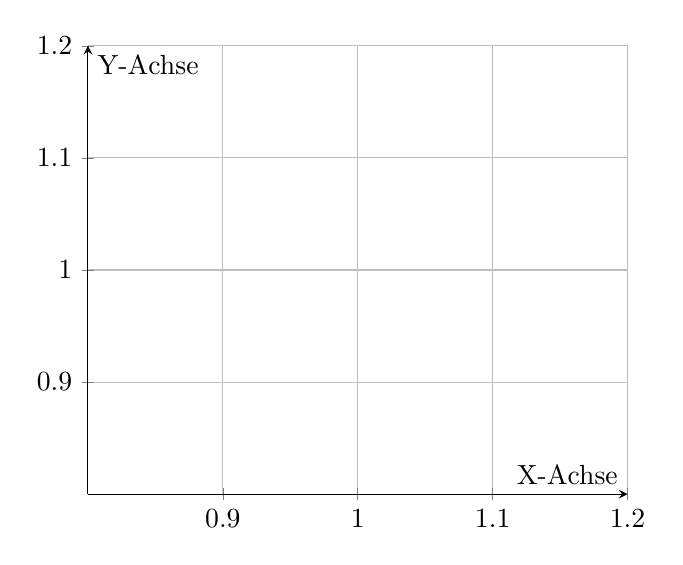
\begin{tikzpicture}
\begin{axis}[
    title={},
    xlabel={X-Achse},
    ylabel={Y-Achse},
    axis lines=middle, % Zentriert die Achsen
    xmin=1, xmax=1, % Setzt die Grenzen für die X-Achse
    ymin=1, ymax=1, % Setzt die Grenzen für die Y-Achse
    grid=major, % Fügt ein Hauptgitter hinzu
]
\end{axis}
\end{tikzpicture}
\caption{}
\end{figure}

\pagebreak
\subsubsection{$k$ - Koeffizent}
Der Faktor $k$ ist ähnlich wie $a$ und bestimmt die Streckung und Stauchung des Graphen, allerdings wird der Graph an der $Y$-Achse gespiegelt, sobald dieser negativ wird. Dies wird begründet durch 
Die Begründung hierfür ist, dass wenn eine Zahl für $k$ eingesetzt wird, bestimmt $k$ wie oft $x$ multipliziert wird. Hierdurch erreicht der Graph schneller die selben $Y$-Wert für $k>0$. Ist $k<0$, so kehrt sich der Graph um aufgrund der Negätivität von $k$. Werden nun postive Werte für $x$ eingesetzt, so entstehen hierraus immernoch negative Zahlen, denn $-$ mal $+$ ergibt $-$. Somit werden die gleichen $Y$-Werte wie im Positiven erricht, jedoch im Negativen.
%ToDo Hier fehlt ein Graph mit einem Vergleich
\begin{figure}[h!]
\centering
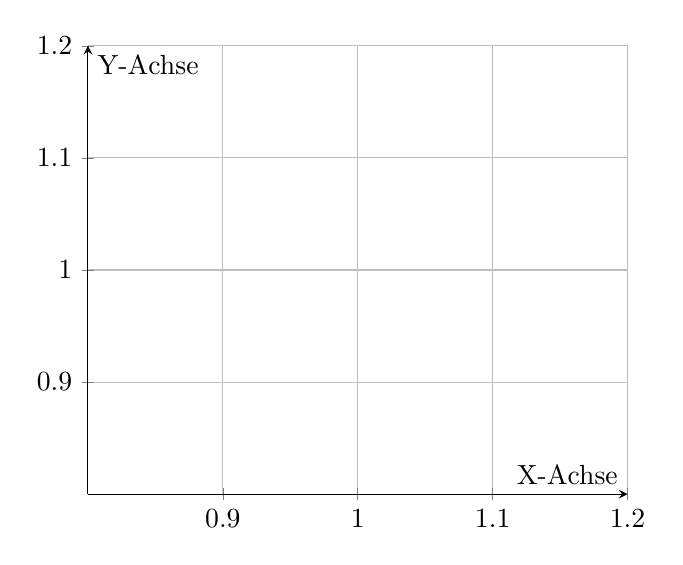
\begin{tikzpicture}
\begin{axis}[
    title={},
    xlabel={X-Achse},
    ylabel={Y-Achse},
    axis lines=middle, % Zentriert die Achsen
    xmin=1, xmax=1, % Setzt die Grenzen für die X-Achse
    ymin=1, ymax=1, % Setzt die Grenzen für die Y-Achse
    grid=major, % Fügt ein Hauptgitter hinzu
]
\end{axis}
\end{tikzpicture}
\caption{}

\end{figure}
\pagebreak
\subsubsection{$d$ - $X$-Achsenverschiebung}
Die Variable $d$ gibt die $X$-Achsenverschiebung an. Sei $d>0$ verschiebt sich der Graph nach links, andernfalls für $d<0$ verschiebt sich der Graph nach rechts. 
%ToDo Hier fehlt ein Graph mit einem Vergleich
\begin{figure}[h!]
\centering
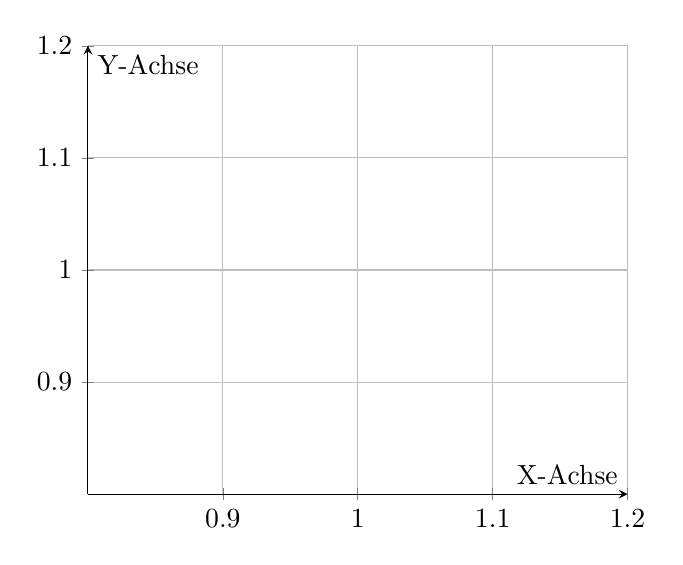
\begin{tikzpicture}
\begin{axis}[
    title={},
    xlabel={X-Achse},
    ylabel={Y-Achse},
    axis lines=middle, % Zentriert die Achsen
    xmin=1, xmax=1, % Setzt die Grenzen für die X-Achse
    ymin=1, ymax=1, % Setzt die Grenzen für die Y-Achse
    grid=major, % Fügt ein Hauptgitter hinzu
]
\end{axis}
\end{tikzpicture}
\caption{}

\end{figure}

\pagebreak
\subsubsection{$c$ - $Y$-Achsenverschiebung}
Der Summand $c$ bestimmt die $Y$-Achsenverschiebung. Dies ist begründet durch die Tatsache, dass wenn ein Summand zu $x$ addiert wird, dieser immer um $c$ nach oben verschoben ist. 
%ToDo Hier fehlt ein Graph mit einem Vergleich
\begin{figure}[h!]
\centering
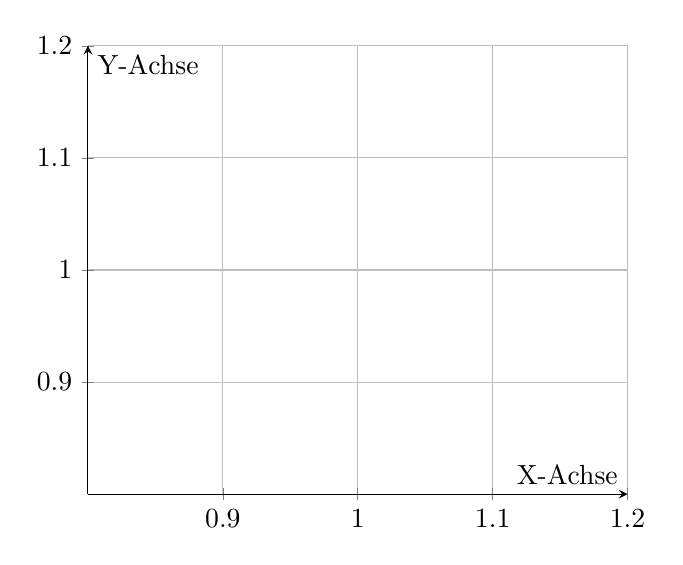
\begin{tikzpicture}
\begin{axis}[
    title={},
    xlabel={X-Achse},
    ylabel={Y-Achse},
    axis lines=middle, % Zentriert die Achsen
    xmin=1, xmax=1, % Setzt die Grenzen für die X-Achse
    ymin=1, ymax=1, % Setzt die Grenzen für die Y-Achse
    grid=major, % Fügt ein Hauptgitter hinzu
]
\end{axis}
\end{tikzpicture}
\caption{}

\end{figure}







% E-Funktion
\pagebreak
\section{$e$-Funktion}\label{sec:e-Funktion}
Die E-Funktion ist einen Unterart der Exponentialfunktion (\ref{sec:Exponentialfunktionen}) sie hat, anders als eine Exponentialfunktion, einen belibige Zahl als Basis. Die Basis einer $e$-Funktion ist die eulischere Zahl $e$. 
\subsection{Entstehung von $e$} \label{sec:E-Funktion/Entstehung von e}
Die Entstehung von $e$ ist ein Grenzwertprozess...
%ToDo Entstehung von e

\subsection{Normalform}\label{sec:E-Funktion/Normalform}
Die Normalform einer $e$-Funktion lautet
\[a\cdot e^{k\cdot x}\]
%TODO Normalform der e-Funktion hinzufügen

\subsection{Ableiten der $e$ Funktion}\label{sec:E-Funktion/Ableiten der e Funktion}
Die besonderheit bei $e$-Funktionen ist, dass die Differenzierte und Integrierte Funktion jeweils immer gleich ist. 
%ToDo Hier fehlen Informationen über das Integrieren und Differenzieren
\subsubsection{Faktorregel}\label{sec:E-Funktion/Normalform} 
Ähnlich wie bei dem normalen Ableiten bei einer ganzrationalen Funktion lässt sich hier die Faktorregel anwenden.
%ToDo Hier fehlen Informationen bezüglich des Ableitens und Differenzieren
\subsubsection{Kettenregel}
Liegt eine verkette Funktion vor, so kann diese mithilfe der Kettenregel abgleitet werden. Bei einer verketteten Funktion gibt es eine äußere Funktion und eine innere Funktion. 
Die Kettenregel ist ein wichtiges Hilfsmittel beim Ableiten von komplexeren Funktion, die sich in eine innere und äußere Funktion einteilen lassen. Die Kettenregel lautet wie folgt.
\begin{align*}
	f(x)&=u(v(x))\\
	f'(x)&=u'(v(x))\cdot v'(x)
\end{align*}
Wobei $u(x)$ die äußere Funktion darstellt und $v(x)$ die äußere Funktion. 
Um mit der Kettenregel zu integrieren wendet man folgende Normalform an. 
\begin{align*}
	f(x)=u(v(x))\\
	F(x)=\frac{U(v(x))}{v'(x)}
\end{align*}
\begin{beispiel}
	\begin{align*}
		f_1(x)=e^{\frac{1}{2}x}\tag{Aufteilen in innere- und äußere Funktion}\\
		v(x)=\frac{1}{2}x \tag{Die innere Funktion}\\
		u(x)=e^x\tag{Die äußere Funktion}\\
	\end{align*}
	Anschließend werden die Funktionen einzeln abgleitet und wieder mit der Form zusammen gebracht.
\end{beispiel}
\subsubsection{Differentialgleichungen}
Differentialgleichungen werden vorwiegend genutzt, um eine gesuchte Funktion mit einer Gleichung zu erhalten. Konkret bedeutet dies, dass eine Differentialgleichung 1. Ordnung
die Ausgangsfunktion und die Ableitung enthält. Allerdings bezieht sich dies nur auf e-Funktionen. So kann man beispielsweise eine e-Funktion wie folgt ableiten. 

\begin{beispiel}
	\begin{align*}
		f'(x)=k\cdot f(x)\\
	\end{align*}
In der Anwendung von Differnetialgleichungen gibt es außerdem noch die Möglichkeit Bedingungen aufzustellen ($f(0)=1$). Mit solchen Bedingungen kann man wie folgt umgehen.

\begin{beispiel}
\begin{align*}
	f(0)=1\tag{Bedingung}\\
	f(0)=e^{k\cdot 1}\tag{Nach $k$ auflösen}\\
	ln(f(0))=k\cdot 1\tag{Dividieren durch 1}\\
	ln(f(0))=k\\
	\Rightarrow f'(x)=ln(f(0))\cdot f(x)
\end{align*}
\end{beispiel}

\subsection{$e$-Funktion aufstellen}
Um eine $e$-Funktion aufzustellen aus einem gegeben Sachverhalt, ist mindestens ein Wertepaar in der $(F;G)$ notwendig. Hierfür nimmt man zu Beginn die Normalform der $e$-Funktion ($ae^{kx}$)
\begin{align}
	f(x)&=ae^{kx}\\
	G&=ae^{kF}\\
	\frac{G}{a}&=e^{kF}\\
	ln\left(\frac{G}{a}\right)&=kF\\
	\frac{ln\left(\frac{G}{a}\right)}{F}&=k
\end{align}
\subsubsection{Erklärung}
Durch die Tatsache, dass ein Wertepaar gegeben ist und dies in die Form einer $e$-Funktion eingesetzt werden kann und somit für eine unbekannte Variable gesorgt wird, ist es möglich dies mithilfe des Logarithmus aufzulösen.
\begin{enumerate}
	\item Die Normalform der $e$-Funktion
	\item Das Wertepaar wird in die Normalform der $e$-Funktion eingesetzt
	\item Der Koeffizent wird durch Division auf die andere Seite gebracht. 
	\item Durch die Tatsache, dass der Logarithmus die Beziehung zwischen dem Ergebnis einer Potenzierung mit einem unbekannten Exponenten darstellt und $e$ in diesem Fall unsere Basis ist, dessen Exponenten genau die links neben dem Gleichheitszeichen ergibt. 
\end{enumerate}

\begin{beispiel}
	Gesucht ist die Funktion $f$. Diese soll mithilfe von der Normalform der $e$-Funktion aufgestellt werden. Der hierfür benötigte Punkt lautet $(5;12)$
	\begin{align*}
		f(x)&=ae^{kx}\\
		12&=e^{k5}\tag{Anwenden des ln}\\
		ln(12)&=k5\tag{Dividieren mit 5}\\
		\frac{ln(12)}{5}&=k\\
		f(x)&=e^{x\cdot \frac{ln(12)}{5}}
	\end{align*}
\end{beispiel}
\pagebreak
\subsection{Umformung von der normalen Exponentialfunktion zu der E-Funktion}\label{sec:E-Funktion/Umformung von der normalen Exponentialfunktion zu der E-Funktion}
Da sich die $e$-Funktion besonders gut differenzieren und integrieren lässt, nutzt man diese, um Sachverhalte darzustellen. Hierfür formt man die normale Exponentialfunktion so um, dass man sie als $e$-Funktion schreiben kann. Hierfür ist es relevant die Bedeutung der folgenden Normalform zu kennen. 
\subsubsection{Normalform}\label{sec:E-Funktion/Umformung von der normalen Exponentialfunktion zu der E-Funktion/Normalform}
\begin{align*}
	f(x)=a\cdot e^{k\cdot x+d}+c
\end{align*}
\geogebra{https://www.geogebra.org/m/bkar24wm}
\pagebreak
\subsubsection{$a$ - Streckfaktor}\label{sec:E-Funktion/Umformung von der normalen Exponentialfunktion zu der E-Funktion/Normalform/a - Streckfaktor}
Der Faktor $a$ ist bestimmt die Streckungs/Stauchungs des Graphen. Wird dieser negativ, so wird der Graph an der $X$-Achse gespiegelt. Der Grund hierfür ist, dass ist $a$ negativ, werden die gesamten Werte des Graphen ebenfalls negativ. 
%ToDo Hier fehlt ein Graph mit einem Vergleich
\begin{figure}[h]
\centering
	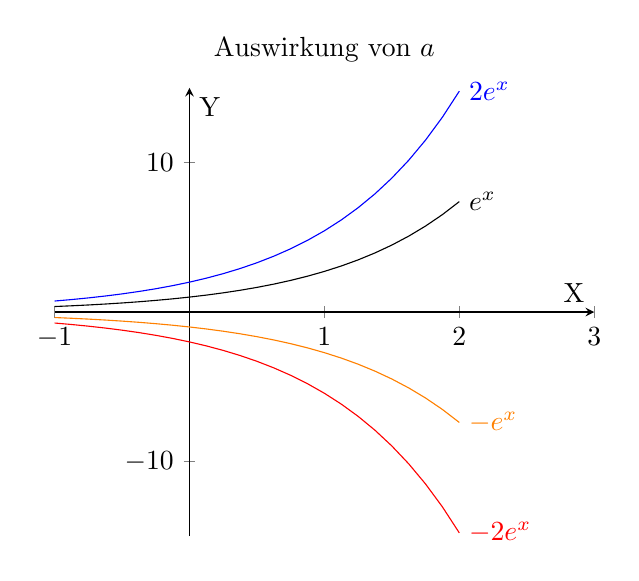
\begin{tikzpicture}
		\begin{axis}[
		title={Auswirkung von $a$},
		axis lines=middle,
		clip=false,
		xlabel={X},
		ylabel={Y},
		xmin=-1,
		xmax=3,
		ymin=-15,
		ymax=15
		]
		\addplot[domain=-1:2,blue]{2*exp(x)} node[right,pos=1]{$2e^x$};
		\addplot[domain=-1:2,black]{exp(x)}node[right,pos=1]{$e^x$};
		\addplot[domain=-1:2,orange]{-exp(x)}node[right,pos=1]{$-e^x$};
		\addplot[domain=-1:2,red]{-2*exp(x)}node[right,pos=1]{$-2e^x$};
		\end{axis}
	\end{tikzpicture}
	\caption{Auswirkung von $a$ auf den Graphen}
\end{figure}
\pagebreak
\subsubsection{$k$ - Koeffizent} \label{sec:e-Funktion/Umformung von der normalen Exponentialfunktion zu der E-Funktion/Normalform/k - Koeffizent}
Der Faktor $k$ ist ähnlich wie $a$ und bestimmt die Streckung und Stauchung des Graphen, allerdings wird der Graph an der $Y$-Achse gespiegelt, sobald dieser negativ wird. Dies wird begründet durch 
Die Begründung hierfür ist, dass wenn eine Zahl für $k$ eingesetzt wird, bestimmt $k$ wie oft $x$ multipliziert wird. Hierdurch erreicht der Graph schneller die selben $Y$-Wert für $k>0$. Ist $k<0$, so kehrt sich der Graph um aufgrund der Negätivität von $k$. Werden nun postive Werte für $x$ eingesetzt, so entstehen hierraus immernoch negative Zahlen, denn $-$ mal $+$ ergibt $-$. Somit werden die gleichen $Y$-Werte wie im Positiven erricht, jedoch im Negativen.
%ToDo Hier fehlt ein Graph mit einem Vergleich
\begin{figure}[h]
\centering
	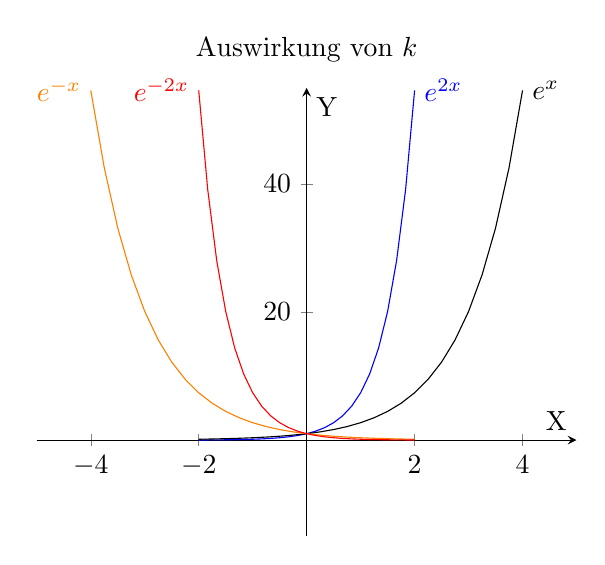
\begin{tikzpicture}
		\begin{axis}[
		title={Auswirkung von $k$},
		axis lines=middle,
		clip=false,
		xlabel={X},
		ylabel={Y},
		xmin=-5,
		xmax=5,
		ymin=-15,
		ymax=55
		]
		\addplot[domain=-2:2,blue]{exp(2*x)} node[right,pos=1]{$e^{2x}$};
		\addplot[domain=-2:4,black]{exp(1*x)}node[right,pos=1]{$e^x$};
		\addplot[domain=-4:2,orange]{exp(-1*x)}node[left,pos=0]{$e^{-x}$};
		\addplot[domain=-2:2,red]{exp(-2*x)}node[left,pos=0]{$e^{-2x}$};
		\end{axis}
	\end{tikzpicture}
	\caption{Auswirkung von $k$ auf den Graphen}
\end{figure}


\pagebreak
\subsubsection{$d$ - $X$-Achsenverschiebung}\label{sec:E-Funktion/Umformung von der normalen Exponentialfunktion zu der E-Funktion/Normalform/d - X-Achsenverschiebung}
Die Variable $d$ gibt die $X$-Achsenverschiebung an. Sei $d>0$ verschiebt sich der Graph nach links, andernfalls für $d<0$ verschiebt sich der Graph nach rechts. 
%ToDo Hier fehlt ein Graph mit einem Vergleich
\begin{figure}[h]
\centering
	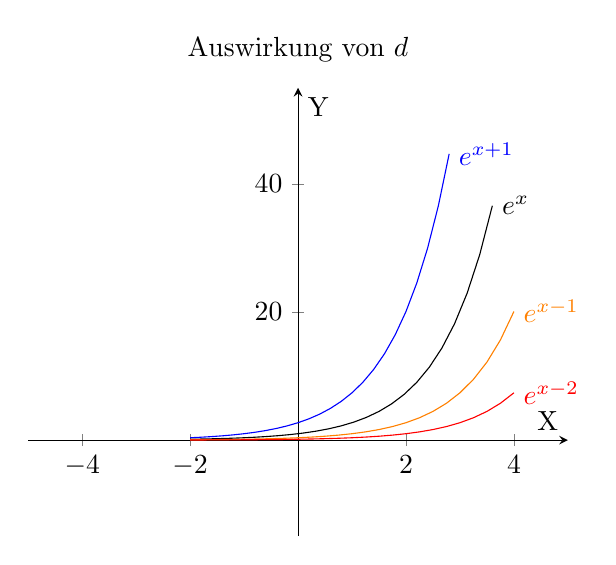
\begin{tikzpicture}
		\begin{axis}[
		title={Auswirkung von $d$},
		axis lines=middle,
		clip=false,
		xlabel={X},
		ylabel={Y},
		xmin=-5,
		xmax=5,
		ymin=-15,
		ymax=55
		]
		\addplot[domain=-2:2.8,blue]{exp(x+1)} node[right,pos=1]{$e^{x+1}$};
		\addplot[domain=-2:3.6,black]{exp(x)}node[right,pos=1]{$e^x$};
		\addplot[domain=-2:4,orange]{exp(x-1)}node[right,pos=1]{$e^{x-1}$};
		\addplot[domain=-2:4,red]{exp(x-2)}node[right,pos=1]{$e^{x-2}$};
		\end{axis}
	\end{tikzpicture}
	\caption{Auswirkung von $d$ auf den Graphen}
\end{figure}

\pagebreak
\subsubsection{$c$ - $Y$-Achsenverschiebung}\label{sec:e-Funktion/Umformung von der normalen Exponentialfunktion zu der E-Funktion/Normalform/c - Y-Achsenverschiebung}
Der Summand $c$ bestimmt die $Y$-Achsenverschiebung. Dies ist begründet durch die Tatsache, dass wenn ein Summand zu $x$ addiert wird, dieser immer um $c$ nach oben verschoben ist. 
\begin{figure}[h]
\centering
	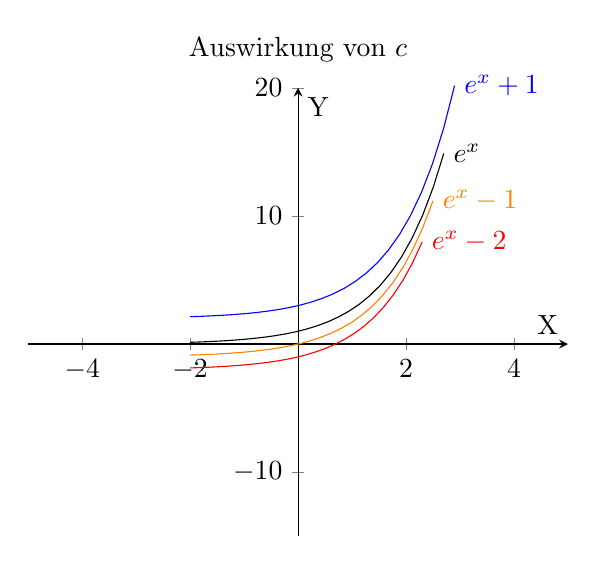
\begin{tikzpicture}
		\begin{axis}[
		title={Auswirkung von $c$},
		axis lines=middle,
		clip=false,
		xlabel={X},
		ylabel={Y},
		xmin=-5,
		xmax=5,
		ymin=-15,
		ymax=20
		]
		\addplot[domain=-2:2.9,blue]{exp(x)+2} node[right,pos=1]{$e^{x}+1$};
		\addplot[domain=-2:2.7,black]{exp(x)}node[right,pos=1]{$e^x$};
		\addplot[domain=-2:2.5,orange]{exp(x)-1}node[right,pos=1]{$e^{x}-1$};
		\addplot[domain=-2:2.3,red]{exp(x)-2}node[right,pos=1]{$e^{x}-2$};
		\end{axis}
	\end{tikzpicture}
	\caption{Auswirkung von $c$ auf den Graphen}
\end{figure}
\pagebreak
\subsection{Umschreiben einer Exponentialfunktion zu einer $e$-Funktion}
Das Umschreiben einer normalen Exponentialfunktion in eine $e$-Funktion erfolgt systematisch nach folgenden Schritten. Allerdings ist dies nur andwendbar auf bereits bestehenden Exponentialfunktionen.
\begin{enumerate}
	\item Eine Funktion ist geben mit dem Funktionsterm $ab^x$
	\item $a$ bleibt stehen
	\item anstelle von $b^x$ wird $e$ geschrieben
	\item Als Exponent wird nun der $\mathrm {ln}(b^x)$ geschrieben. 
\end{enumerate}
Bedeutet, dass \[a\cdot b^x=a\cdot e^{ln(b^x)}\]

\subsection{Verdopplungszeit und Halbwertszeit einer $e$-Funktion bestimmen.}
Liegt eine Funktion mit $e$ als Basis vor, so kann man die Verdoppelungszeit oder die Halbwertszeit bestimmen, indem man die folgende Formel anwendet
\[x=\frac{ln(2)}{k}\]
Hierbei ist $k$ die Wachstumskonstante und $x$ die Zeit. Für die Halbwertszeit gilt die folgende Formel.
\[x=\frac{ln(0.5)}{k}\]
Wobei die $x$ die Zeit darstellt, $k$ die Wachstumskonstante und $ln(0.5)$ die Halbierung
%ToDo Hier fehlt eine Begründung









\end{document}